\documentclass[12pt]{report}
%\usepackage{fancyvbr, pstcol}
%\setlength{\parskip}{1ex plus 0.5ex minus 0.2ex}
\setlength{\parskip}{1em}
\parindent0mm
\textwidth150mm
\textheight200mm
\oddsidemargin+5mm

\usepackage[pdftex]{graphicx}
\usepackage{color}
\usepackage{amsfonts}
\usepackage{longtable}

\definecolor{LightBlue}{rgb}{0.8,0.85,1}
\definecolor{Light}{gray}{.85}
\setlength{\fboxrule}{1pt}
\setlength{\fboxsep}{2pt}
\setlongtables

\newcommand{\vect}[1]{\ensuremath{\mathrm{\mathbf{#1}}}}
\newcommand{\pdiv}[2]{\ensuremath{\frac{\partial #1}{\partial #2}}}
\newcommand{\WarningBox}[1]{
  %\fcolorbox[rgb]{0,0,0}{0.95,0.95,0.95}{
    \fcolorbox{black}{Light}{
    \begin{minipage}{0.965\linewidth}
      \textbf{WARNING:}
      #1
    \end{minipage}
  }
}

\newcommand{\ImportantBox}[1]{
  %\fcolorbox[rgb]{0,0,0}{0.95,0.95,0.95}{
    \fcolorbox{black}{LightBlue}{
    \begin{minipage}{0.965\linewidth}
      \textbf{IMPORTANT:}
      #1
    \end{minipage}
  }
}

\begin{document}

%Cover page
\thispagestyle{empty}	%don't include number on cover
%\begin{flushleft}
%\begin{figure}
%
\includegraphics[width=0.3\textwidth]{IHPC-logo.pdf}
%\end{figure}
%\end{flushleft}
\verb+ +
\vspace{4cm}
\begin{flushright}
\huge\bf depSolver v2.1\\
\rule{\textwidth}{4pt}
\large{\bf Document Revision 1.0\\
\today}
\end{flushright}

%Back of cover page (copyright)
\newpage
\thispagestyle{empty}
\begin{flushleft}
\begin{figure}
\includegraphics[width=0.2\textwidth]{gplv3-127x51.png}
\end{figure}
\section*{}
\vspace{10cm}
Carlos Rosales Fern\'andez\\
\verb+carlos@ihpc.a-star.edu.sg+\\
\vspace{0.5em}
Heterogeneous Coupled Systems Team\\
Large-Scale Complex Systems\\
Institute of High Performance Computing\\
1 Science Park Road, \#01-01 The Capricorn\\
Science Park II, Singapore 117528\\
\vspace{1cm}
Copyright \copyright  2006, 2008 Carlos Rosales Fern\'andez and the Institute of High Performance Computing, Singapore.
\end{flushleft}
\newpage

\pagenumbering{roman}	%for preface sections only
\section*{Preface}\noindent \verb+depSolver+ is a Boundary Element Method solver for Laplace's equation in 3D AC electrostatic problems. I originally wrote this program to study the characteristics of different dielectrophoretic trap designs. A big advantage of using this code to calculate dielectrophoretic forces is that the user can specify which approximation to use for the calculation of the force. In this manner, without having to change anything in the code, one can use a simple dipolar or quadrupolar approximation to quickly explore the force generated on a sphere over a large volume of space, or use the more general calculation based on the integration of the Maxwell's stress tensor over an arbitrarily shaped particle. An example of research work done with this code is reference \cite{Rosales2005}.

\noindent \verb+depSolver+ is convenient for dielectrophoretic force calculations, but it is in no way limited to them. It can be used to solve a wide variety of electrostatic problems as long as they involve conductors were the electric potential is specified and all dielectrics in the system can be considered as piecewise homogeneous. The source code is written in C and uses separate functions for most tasks in order to make modifications easier.

\noindent Changes in Version 2.0 of depSolver are related to the code structure and the output options:

\begin{enumerate}
\item Strings read from the input file now have limited size to avoid the possibility of stack overflow.
\item Header style now matches most OSS projects. This should make modification of the code easier.
\item Related functions are now grouped in files shorter than 1000 lines. This is also to facilitate code modification and maintenance.
\item A new output option is available with a format accepted by Paraview\cite{Paraview}. Visualization of the potential and the field is now much easier.
\end{enumerate}

\noindent This manual consists of three parts: Part I describes how to prepare the inputs necessary for the program and how to post-process the solution; Part II describes the indirect formulation of the BEM for those interested in the details, and Part III gives details on the implementation. In order to use the code you striclty only need to read Part I, but I recommend anyone using the program to calculate dielectrophoretic forces to go through Chapter 9 in Part III of this document. Part II has been included because most people are not familiar with the indirect formulation of the BEM, but you can safely ignore it if this does not apply to you.

\noindent The Institute of High Performance Computing (IHPC) distributes \verb+depSolver+ under a dual licensing policy. We believe in open source software for pushing the frontiers of science and engineering, and we encourage everyone to publish open source software under the GPL License. You are free to use, copy, modify and distribute any element of \verb+depSolver+ under the GNU General Public License version 3. IHPC also provides a flexible OEM Commercial License for OEMs, ISVs, and VARs.

\noindent Finally, although the GPL License does not require you to contact us, I would appreciate if you could send an email telling me that you are using \verb+depSolver+ and what application you are using the code for.

\noindent The complete package can be downloaded from \verb+software.ihpc.a-star.edu.sg+.

\vspace{1cm}
	Carlos Rosales Fern\'andez\\
	Singapore, \today

\tableofcontents
\pagebreak
\section*{}
\pagebreak

\pagenumbering{arabic}	%for preface sections only
\part{User Manual}

\pagebreak
\section*{}
\pagebreak

\chapter{Introduction and general remarks}
\verb+depSolver+ is distributed as a series of C function files, a make file for compilation, a Patran \cite{patran} script for mesh generation called \verb+bem_save.pcl+, and tools to modify the output files to set them in formats which are easily plotted in Matlab \cite{matlab} or gnuplot \cite{gnuplot}. The complete list of functions is collected in Appendix A.

\section{Quick Install Guide}
This is for those of you in a hurry. Unzip \verb+depSolver-2.0.tar.gz+ in a suitable directory:

\begin{tabular}{l}
\texttt{\$ tar -zxvf depSolver-2.0.tar.gz}
\end{tabular}

then type:

\begin{tabular}{l}
\texttt{\$ ./install.sh}
\end{tabular}

Assuming you have working versions of \verb+gcc+, \verb+make+, and \verb+doxygen+ this will give you a full installation of depSolver.


\section{Complete Install Guide}
Unzip the \verb+depSolver-2.0.tar.gz+ file in a suitable directory. This can be done in a linux system by typing on the command line:

\begin{tabular}{l}
\texttt{\$ tar -zxvf depSolver-2.0.tar.gz}
\end{tabular}

or alternatively using two separate commands:

\begin{tabular}{l}
\texttt{\$ gunzip depSolver-2.0.tar.gz}\\
\texttt{\$ tar -xvf depSolver-2.0.tar}
\end{tabular}

The following directories will be created:

\begin{tabular}{ll}
\texttt{depSolver}&: Main program directory\\
\texttt{depSolver/bin}&: Directory where the binary files are stored after compilation\\
\texttt{depSolver/docs}&: Directory containing the code documentation\\
\texttt{depSolver/examples}&: Directory with examples to test the compiled code\\
\texttt{depSolver/src}&: Directory containing the C source code\\
\texttt{depSolver/utils}&: Directory with utilities for pre- and post-processing\\
\texttt{utils/depBreak}&: Utility to break data files into several units\\
\texttt{utils/fieldPost}&: Utility to format the field values for plotting in matlab\\
\texttt{utils/forcePost}&: Utility to format the force values for plotting in matlab\\
\texttt{utils/gplotFormat}&: Utility to format standard output files for 3D plotting in gnuplot with pm3d\\
\texttt{utils/meshgen-std}&: Utility to generate planes of points for post-processing\\
\texttt{utils/meshgen-vtk}&: Utility to generate points for post-processing with Paraview\\
\texttt{utils/p2b }&: Utility to transform mesh from Patran format\\
\texttt{utils/potPost}&: Utility to format the potential values for plotting in matlab\\
\end{tabular}

In order to install and run \verb+depSolver+ all the \verb+.c+ and \verb+.h+ listed in appendix A are necessary. Make sure all the mentioned files are inside the \verb+depSolver/src+ directory. Then type:

\begin{tabular}{l}
\texttt{\$ ./install.sh}
\end{tabular}

This will install \verb+depSolver+, all the utilities and the documentation provided you have working installations of \verb+gcc+, \verb+make+ and \verb+Doxygen+ \cite{doxygen}. An install log and an install error file will be generated. You will be informed of the success/failure of the installation both on screen and in the installation log.

If Doxygen is not installed in your system a warning will be presented but the installation will be considered successful, as this is only required for the Reference Manual documentation only. The User Manual is a pdf file that is always provided with the distribution and it is independent of the presence of Doxygen in your system, so the instructions on the usage of depSolver will always be available.

\subsection{Individual Compilation}
Two versions of the code can be compiled. The basic version is called \verb+depSolver+, and an additional version called \verb+depSolver-sft+ is also provided. Both versions of the code are identical except that in \verb+depSolver-sft+ it is assumed that a particle - which can be of any shape - is created in the geometry and the program will shift it as a rigid body following a vector given in the input file. Notice that this shift assumes that the particle is created at the center of coordinates. This version is useful to produme Maxwell Stress Tensor calculations of the dielectrophoretic force without having to create a new mesh for each particle position. It can be abused to work without a particle or using a zero displacement, but the basic \verb+depSolver+ is less confusing to use in those cases.

A makefile is provided for the compilation of the code. Inside \verb+depSolver/src+ type:

\begin{tabular}{l}
\texttt{\$ make depSolver \&\& make install}
\end{tabular}

or

\begin{tabular}{l}
\texttt{\$ make depSolver-sft \&\& make install}
\end{tabular}

This will compile using gcc with the flag -O3 and several other performance optimization flags. If for some reason you don't like this, or you would like to add an architecture-related flag simply change the makefile. The executable files are automatically saved to \verb+depSolver/bin+.

To clean the directory of object files after the compilation, type the following:

\begin{tabular}{l}
\texttt{\$ make clean}
\end{tabular}

\subsection{Running the solver}
In order to run \verb+depSolver+ certain input files are needed. These files have the extension \verb+.bem+ and the ones needed for every run are:

\begin{tabular}{ll}
\texttt{input.bem}&: Main input file\\
\texttt{nodes.bem}&: File containing the coordinates of the nodes in the mesh\\
\texttt{elems.bem}&: File containing the element connectivity of the mesh\\
\texttt{bcs.bem}&: File containing the boundary conditions at every node
\end{tabular}

There are also two optional files files which are only used for some calculations: 

\begin{tabular}{ll}
\texttt{forcepoints.bem}&: [opt] File containing the points where the force is\\
  & \verb+ + calculated when using the multipolar approximation\\
\texttt{internal.bem}&: [opt] File containing the internal points where the\\
  & \verb+ + potential or field (or both) are required
\end{tabular}

Notice that the names of all these files are read from \verb+input.bem+ and can be changed at will. Only the main input file \verb+input.bem+ must keep this name as it is hard coded. Once these files have been properly set -- see the following section for details on the format and contents --, one can simply run \verb+depSolver+ in the background, since all output is directed to files and there is no interaction with the program while it runs. The output files generated by the program are also divided in those that are produced on every run:

\begin{tabular}{ll}
\texttt{bem.log}&: Main log file, logs program advance and execution time\\
\texttt{solution.dat}&: Solution in the format \texttt{x y z Re[s] Im[s]}
\end{tabular}

And those that are produced only for certain input options:

\begin{tabular}{ll}
\texttt{gmres.log}&: [opt] GMRES log file, registers the error per iteration\\
\texttt{field.dat}&: [opt] Contains the electric field at the required points\\
\texttt{force-mp.dat}&: [opt] Contains the DEP force (multipolar approximation)\\
\texttt{formce-mst.dat}&: [opt] Contains the DEP force (Maxwell's stress tensor method)\\
\texttt{potential.dat}&: [opt] Contains the potential at the required points\\
\end{tabular}
\pagebreak

\chapter{Pre-Processing}
This chapter describes how to set up the necessary input files.

\section{Mesh Generation Using Patran}
To generate the mesh and the boundary conditions using Patran, simply generate the geometry using a structural model and ensuring that the normals are outward-facing (otherwise go to {\it Elements} and use {\it Modify$\rightarrow$Element$\rightarrow$Reverse}).

Then go to {\it Loads} and use the {\it Displacement} type to set the boundary conditions in the conductors in the system as:

\begin{tabular}{l}
\texttt{< 1 Re[V] 0 >}\\
\texttt{< 1 Im[V] 0 >}
\end{tabular}

The first number (1) indicates the potential is given, and the last number can be anything, because it is not used.

Next, use the {\it Force} type to set the boundary conditions in the interfaces as:

\begin{tabular}{l}
\texttt{< 0 0 interfaceID >}\\
\texttt{< 0 0 interfaceID >}
\end{tabular}

In this case it is important that the first two values are zero, since they are the type of boundary condition - the value of \verb+vBCType[]+ in the code - and the right hand side of the boundary equation - the value of \verb+vB[]+ in the code.

Once this is done run the command \verb+!!input bem_save.pcl+ in Patran's command line, and make sure that you receive a message saying that the compilation has been successful (this should be instantaneous). Then run \verb+bem_save()+ in the same command line of Patran. This saves the nodes, elements and boundary conditions in the files \verb+nodes.out+, \verb+elems.out+ and \verb+bcs.out+, and also stores information about the mesh - number of nodes, elements and nodes per element - in the file \verb+mesh_info.out+.

\section{Converting Patran output to the right format}
In order to get the input files in the exact format needed for the \verb+depSolver+ executable a further step is necessary. Go to the directory called \verb+depSolver/utils/p2b+ and run:

\begin{tabular}{l}
\texttt{\$ ./p2b elemType scaling}
\end{tabular}

This needs the output files from Patran, \verb+nodes.out+, \verb+elems.out+ and \verb+bcs.out+, and yields the correctly formatted \verb+nodes.bem+, \verb+elems.bem+ and \verb+bcs.bem+.

This last step seems a bit unnecessary, but Patran uses a different order for the quadratic elements than \verb+depSolver+, and setting the parameter \verb+reOrder+ to one transforms the element connectivity to the appropriate format for the program. It is  also handy when one needs to test the same system but scaled at different sizes, because no re-meshing is necessary. Additionally this filter takes care of repeated nodes in the mesh left by Patran, and updates the corresponding references in the element connectivity file, resulting in a more stable system of equations (otherwise there would be repeated equations in the coefficient matrix, making the system not solvable!).

Full help can be obtained on screen by calling the program as: \texttt{./p2b -h}.

\section{Generating evaluation points file}\label{meshgen-std}
\subsection{Standard Output}
Inside \verb+depSolver/utils/meshgen+ there is an executable file that generates sets of points in constant planes. This is useful to generate the \verb+internal.bem+ and \verb+forcepoints.bem+ files. It is called as:

\begin{tabular}{l}
\texttt{\$ ./meshgen-std firstLine nx ny nz n rmin rmax r}
\end{tabular}

This generates a regular 2D mesh with limits [(\verb+xmin+,\verb+xmax+):(\verb+ymin+,\verb+ymax+)] in the plane
\verb+constantPlane+ = \verb+r+, where \verb+constantPlane+ takes the values \verb+x+, \verb+y+ or \verb+z+.

Example of use:

\begin{tabular}{l}
\texttt{\$ ./meshgen-std 1 z 100 20 -50 50 -10 10 0.0 1}
\end{tabular}

Produces a mesh in the plane z = 0.0 in the range x = (-50,50), y = (-10,10), with 100 points in the x direction and 20 in the y direction. The line number is saved to the ouput file starting with 1.

The output file is called 'mesh.dat' for convenience. It can be called sucesively in order to produce a single file with all the necessary points, as long as \verb+firstLine+ contains the correct number of the first element of the plane for each call. If a 21x21 set of points is being generated the first call will be done with \verb+a+ = 1, the second with \verb+a+ = 442, etc \ldots

Full help can be obtained on screen by calling the program as: \texttt{./meshgen-std -h}.

\subsection{Paraview Formatted Output}
Inside \verb+depSolver/utils/meshgen-vtk+ there is an executable file that generates sets of points in a given volume. This is useful to generate the \verb+internal.bem+ files with a VTK format, which can be read by Paraview. It is called as:

\begin{tabular}{l}
\texttt{\$ ./meshgen-vtk nx ny nz xmin xmax ymin ymax zmin zmax}
\end{tabular}

This generates a regular 3D mesh with limits [(\verb+xmin+,\verb+xmax+):(\verb+ymin+,\verb+ymax+):(\verb+zmin+,\verb+zmax+)]

Example of use:

\begin{tabular}{l}
\texttt{\$ ./meshgen-vtk 20 20 10 -50 50 -25 25 0 10}
\end{tabular}

Produces a regular cartesian grid with 4000 points in the range x = (-50,50), y = (-25,25), z = (0,10). The line number is saved to the ouput file starting with 1. The two first lines of the file will contain the number of nodes and the spacing between points in each direction respectively.

The output file is called 'mesh.dat' for convenience.

Full help can be obtained on screen by calling the program as: \texttt{./meshgen-vtk -h}.

\pagebreak
\section*{}
\pagebreak

\chapter{Input File Format}
The main input file, \verb+input.bem+, is divided in several sections, each of them with a title to increase readability. C++ style comments are allowed in the file, either occupying a line of their own or situated after the data in a line. The same kind of comments may be included in any of the other \verb+.bem+ files. Blank lines can be used to make the file easier to read.

\section{Nodes Section}
The title \verb+NODES+ is typically used for this section of the file, as it contains the total umber of nodes in the mesh and the name of the file with the nodes positions and indexes. This section should look like:

\begin{tabular}{l}
\texttt{NODES}\\
\texttt{nodeNumber}\\
\texttt{nodeFilename}
\end{tabular}

The data file containing the nodes can have any name (up to 32 characters long), such as the mentioned \verb+nodes.bem+, and must be written in the form:

\begin{tabular}{l}
\texttt{nodeID x y z}
\end{tabular}

And the nodes must be sequentially numbered from 1 to \verb+nodeNumber+.

\section{Elements Section}
The title \verb+ELEMENTS+ is usually given to this section, that must contain the total number of elements in the mesh, the type of elements used, and the name of the file containing the element connectivity information. This section should look like:

\begin{tabular}{l}
\texttt{ELEMENTS}\\
\texttt{elemNumber}\\
\texttt{elemType}\\
\texttt{elemFilename}
\end{tabular}

Where \verb+elemType+ can be one of the following:

\begin{tabular}{ll}
\texttt{tria3}&: Linear interpolation in triangles (3-noded triangles)\\
\texttt{tria6}&: Quadratic interpolation in triangles (6-noded triangles)
\end{tabular}

The actual name of the element type can be in uppercase, lowercase, or a mixture of the two, as long as the spelling is correct!

The file containing the element connectivity information must have the following structure:

\begin{tabular}{l}
\texttt{elemID nodeID1 nodeID2	... nodeIDM}
\end{tabular}

Where \verb+M+ is 3 for linear interpolation in triangles and 6 for quadratic interpolation. The elemID must range from 1 to \verb+elemNumber+. Note that all numbers in this file should be integers.

\section{Materials Section}
This section contains the number of materials used in the simulation and the values of the electric conductivity and relative permittivity of each of them, usually under the title \verb+MATERIALS+. This section should look like:

\begin{tabular}{l}
\texttt{MATERIALS}\\
\texttt{matID sigma eps}
\end{tabular}

Where \verb+sigma+ is the conductivity of the material, and \verb+eps+ its relative permittivity.

\section{Interfaces Section}
This sections carries the title \verb+INTERFACES+, and contains the information about the interfaces between different materials in the following format:

\begin{tabular}{l}
\texttt{INTERFACES}\\
\texttt{interfaceNumber}\\
\texttt{interfaceID mat1 mat2}\\
\end{tabular}

Where \verb+mat1+ and \verb+mat2+ are the two materials that interface. No support for three material interfaces is provided in the code or the input files.

\section{Problem Section}
This section is named \verb+PROBLEM+ and contains the frequency of the external field and the name of the file that has the boundary conditions. It looks like this:

\begin{tabular}{l}
\texttt{PROBLEM}\\
\texttt{frequency}\\
\texttt{bcsFilename}
\end{tabular}

The file that contains the boundary conditions must be in the following format:

\begin{tabular}{l}
\texttt{nodeID bcType value1Re value2Re}\\
\texttt{...}\\
\texttt{nodeID bcType value1Im value2Im}\\
\texttt{...}
\end{tabular}

A dielectric interface is indicated by a \verb+bcType+ of 0, a \verb+value1+ of 0, and a \verb+value2+ equal to the \verb+interfaceID+ where the node belongs. All three values must be the same for the real and imaginary parts.

If the dielectric interface belongs to a particle and the force is calculated using the Maxwell Stress tensor method the \verb+bcType+ must be set to 6 in order to differentiate this surface from any other dielectric interfaces in the system. \verb+value1+ and \verb+value2+ must be set to 0 and the \verb+interfaceID+ where the node belongs as for any other dielectric interface.

A dirichlet boundary condition - in this case, potential given on a conductor - is indicated by a \verb+bcType+ of 1, a \verb+value1Re+ equal to the real part of the potential, and a \verb+value1Im+ equal to the imaginary part of the potential. The \verb+value2+ is not used in the code and must be omited from the file.

Notice that in the boundary conditions file the real part of the boundary conditions is written first, so that for N nodes there are 2N rows, the first N with the real components, the last N with the imaginary ones.

The values 2 to 5 for the boundary condition type are not used by the program and may be assigned to other boundary condition types at a later stage.

\section{Re-positioning Section}
This section must only be used with \verb+depSolver-sft+. It contains the first node corresponding to the particle and the displacement vector for the shift:

\begin{tabular}{l}
\texttt{REPOSITION}\\
\texttt{pNode}\\
\texttt{dx dy dz}
\end{tabular}

where \verb+pNode+ is the last node of the mesh before the particle nodes (if the nodes in the electrodes go from 1 to 536 and the nodes in the particle from 537 to 752 we would use \verb+pNode+ = 536. In Patran the particle must be meshed last to use this option correctly. (\verb+dx+,\verb+dy+,\verb+dz+) are the displacements in each of the spatial directions. 

\section{Analysis Section}
This is the most complicated section in the input file. It is usually titled \verb+ANALYSIS+, and contains al the information relative to which solver to use, and what postprocessing to do with the solution. This section must follow the format below:

\begin{tabular}{l}
\texttt{ANALYSIS}\\
\texttt{solver preCond nInit}\\
\texttt{analysisType}\\
\texttt{pointNumber a b c}\\
\texttt{forceFilename}
\end{tabular}

where \verb+forceFilename+ is the file containing the points where the force is calculated (when using the multipolar approximation), and has the following format:

\begin{tabular}{l}
\texttt{pointID x y z}
\end{tabular}

It is not always necessary to include all these parameters in the section. The particular set of them necessary for a calculation depends on the \verb+solver+ and \verb+analysisType+ requested. Let us examine the section line by line in more detail.

\verb+solver+ can be specified as:

\begin{tabular}{ll}
\texttt{gaussBksb}&: Gauss elimination solver with partial pivoting (columns only),\\
  & \verb+ + does not require the \texttt{preCond} and \texttt{nInit} parameters\\
\texttt{gmres}&: GMRES solver, requires the parameters \texttt{preCond} and \texttt{nInit}
\end{tabular}

The name of the solver can be in lowercase or uppercase. The parameters \verb+preCond+ and \verb+nInit+ must be used only with the GMRES solver. \verb+preCond+ takes value 0 if no pre-conditioning is required and value 1 for Jacobi pre-conditioning (recommended). \verb+nInit+ takes the value 0 if no initial guess is given for the solution, and the number of nodes where the solution is provided otherwise. The file containing the solution must be named \verb+solution.init+, and its format must be:

\texttt{x y z Re[s] Im[s]}

Where \verb+Re[s]+ and \verb+Im[s]+ are the real and imaginary parts of the solution at the point \verb+(x,y,z)+, and the file has \verb+nInit+ rows.

A good practice is to solve the problem of an empty trap first specifying \verb+nInit+ as zero, and then use the solution as initial guess for a trap containing the particle. Note that due to the way the program works one should use exactly the same mesh (apart from the addition of the particle) in both cases. Normally one would generate the mesh for the empty trap, run it, then generate the mesh for the trap with te particle but taking care of meshing in the same order as before, leaving the mesh on the particle surface to the end. This guarantees the program will work correctly. If in doubt set \verb+nInit+ to zero.

The \verb+analysisType+ is an integer that can take the following values:

\begin{tabular}{rl}
0&: Calculate only the potential $\phi$\\
1&: Calculate only the electric field $\vec{E}$\\
2&: Calculate $\phi$ and $\vec{E}$\\
3&: Calculate $\phi$, $\vec{E}$, and $\vec{F}_{\rm DEP}$ using Maxwell's stress tensor method\\
4&: Calculate only $\vec{F}_{\rm DEP}$ using Maxwell's stress tensor method\\
5&: Calculate $\phi$, $\vec{E}$, and $\vec{F}_{\rm DEP}$ using a dipolar approximation on a sphere\\
6&: Calculate $\phi$, $\vec{E}$, and $\vec{F}_{\rm DEP}$ using a quadrupolar approx. on a sphere\\
7&: Calculate $\phi$, $\vec{E}$, and $\vec{F}_{\rm DEP}$ using an octupolar approx. on a sphere\\
8&: Not available (reserved for multipolar approx. of order 4 on a sphere)\\
9&: Not available (reserved for multipolar approx. of order 5 on a sphere)\\
10&: Calculate $\phi$, $\vec{E}$, and $\vec{F}_{\rm DEP}$ using a dipolar approx. for a homogeneous ellipsoid\\
11&: Calculate $\phi$, $\vec{E}$, and $\vec{F}_{\rm DEP}$ using a dipolar approx. for a single-shelled ellipsoid
\end{tabular}

A quadrupolar approximation in this context indicates that dipole + quadrupole terms are included in the calculation, while an octupolar approximation indicates the inclusion of dipolar + quadrupolar + octupolar. When \verb+analysisType+ takes values [0--4] the parameters \verb+(a,b,c)+ do not need to be included in the section. When the value is between 5 and 9 only \verb+a+ has to be specified, and it represents the radius of the spherical particle under consideration. If the calculation of the force is done for an ellipsoid and options 10 or 11 are chosen, all \verb+(a,b,c)+ parameters must be specified, and they represent the three semiaxes of the ellipsoid. 

The parameter \verb+pointNumber+ is only used with options [5--11] and indicates on how many positions of the centre of the sphere/ellipsoid should the force be calculated. The particular positions to use are indicater in the following lines by \verb+(x,y,z)+. If options [1--4] are chosen for the type of analysis neither \verb+pointNumber+ nor these last lines should not be included in the file. 

\section{Internal Points Section}
This section is optional, and only necessary when the potential or the electric field are going to be calculated. It is usually title \verb+INTERNALPOINTS+ and has the following format:

\begin{tabular}{l}
\texttt{INTERNALPOINTS}\\
\texttt{internalPointsNumber outputType}\\
\texttt{internalPointsFilename}
\end{tabular}

Where \verb+outputType+ is either \verb+STD+ (standard output) or \verb+VTK+ (Paraview output). Notice that if the number of internal points is set to zero the output type and the file name do not need to be specified.

\WarningBox{Remember to create the internal node files with the correct version of meshgen, \texttt{meshgen-std} for \texttt{STD} output type and \texttt{meshgen-vtk} for \texttt{VTK}, to avoid unexpected results.}

\verb+internalPointsNumber+ is the total number of rows in the file \verb+internalPointsFilename+, which has the following structure for the \verb+STD+ option:

\begin{tabular}{l}
\texttt{pointID x y z}
\end{tabular}

And the prefered structure is to keep z fixed, y fixed, x fixed, because in this way slices at different constant z are kept separated and are easy to postprocess later on.

The internal nodes file is slightly different for the \verb+VTK+ option:

\begin{tabular}{l}
\texttt{nx ny nz}\\
\texttt{$\Delta$x $\Delta$y $\Delta$z}\\
\texttt{pointID x y z}
\end{tabular}

where \verb+nx+, \verb+ny+, \verb+nz+ are the number of points in each spatial direction; and $\Delta$\verb+x+, $\Delta$\verb+y+, $\Delta$\verb+z+, are the distances between two consecutive points in each direction. This additional information is required by Paraview to render teh data correctly.


\section{Columns Section}
This section is provided in order to be able to calculate properly the electric field and temperature in a channel with cylindrical or square electrode columns. The format is simply:

\begin{tabular}{l}
\texttt{COLUMNS}\\
\texttt{colType}\\
\texttt{nColumns}\\
\texttt{X1 Y1 R1}\\
\texttt{...}\\
\texttt{XnCol YnCol RnCol}
\end{tabular}

where \verb+nColumns+ is the total number of columns in the domain, and \verb+colType+ is the type of column (1 for cylindrical columns, 2 for square columns).

In the case of cylindrical columns \verb+Xi+ and \verb+Yi+ are the positions of the ith column centre and \verb+Ri+ is the radius of the ith column.

In the case of square cross-section columns \verb+Xi+ and \verb+Yi+ are the positions of the ith column centre and \verb+Ri+ is half the side length of the ith column.

If \verb+nColumns+ is zero the rest of the section will be ignored by the program.

\pagebreak
\section*{}
\pagebreak

\chapter{Post-Processing}
This section describes how to use the tools in the \verb+utils+ folder in order to manipulate the program's output. There are four main utilities called \verb+break+, \verb+gplotForm+, \verb+pot-post+ and \verb+field-post+.

\section{Break}\label{break}
This program breaks a single output data file into several independent files. This is useful when the output includes calculations of the potential and the field in several planes and it is necessary to have the results from each plane in an independent file in order to plot them. It resides in \verb+depSolver/utils/breaker+ and must be called as:

\begin{tabular}{l}
\texttt{\$ ./break fileName fileNumber colNumber rowNumber}
\end{tabular}

where \verb+fileName+ is the name of the file to break up, \verb+fileNumber+ is the number of output files, \verb+colNumber+ is the number of columns in the input file, and \verb+rowNumber+ is the number of rows in each of the output files. The output files will be named \verb+data1+, \verb+data2+, ..., \verb+datafileNumber+. The input file is not modified.

If called as \verb+./break -h+ it will print a short help to the screen.

\section{gplotForm}
In the directory \verb+depSolver/utils/gplotFormat+ there is an executable called \verb+gplotForm+ that allows to separate any given data file with an arbitratry number of rows into blocks of a fixed size. This can be used for plotting a set of data corresponding to a plane, for example $z=0$, in gnuplot with the pm3d option. The utility is called as:

\begin{tabular}{l}
\texttt{\$ ./gplotForm filename nRows nBlock nCols}
\end{tabular}

Where \verb+filename+ is the name of the file to separate into blocks, \verb+nRows+ is the total number of rows in the file, \verb+nBlock+ is the size of the blocks to make, and nCols the number of columns in the file. This produces as output the file \verb+temp.gnu+ with the block-separated data that has a blank line every nBlock lines of the original file.

Let's assume that we generated the internal points file using the utility \verb+meshgen+ described in section [\ref{meshgen}], and that we asked meshgen to generate 100 points in the x direction and 20 in the y direction as in the example of use given. Because the total number of points is $100\times20=2000$ and we only have 4 columns (x,y,z,T) in the temperature data file we call separate as:

\begin{tabular}{l}
\texttt{\$ ./gplotForm potential.dat 2000 20 4}
\end{tabular}

The output file can be now used in gnuplot to produce a density plot. First run gnuplot by calling it from the command line:

\begin{tabular}{l}
\verb+$ gnuplot+
\end{tabular}

Once inside gnuplot type:

\begin{tabular}{l}
\texttt{gnuplot> set pm3d}\\
\texttt{gnuplot> splot 'temp.gnu' u 1:2:3:4 w pm3d}
\end{tabular}

if you only want a xy surface plot then use instead:

\begin{tabular}{l}
\texttt{gnuplot> set pm3d map}\\
\texttt{gnuplot> splot 'temp.gnu' u 1:2:4 w pm3d}
\end{tabular}

If called as \verb+./gplotForm -h+ it will print a short help to the screen.

\section{FieldPost}
To process the file \verb+field.dat+ you must go into directory \verb+depSolver/utils/fieldPost+ and run:

\begin{tabular}{l}
\texttt{\$ ./fieldPost nx ny nxi nyi}
\end{tabular}

Where \verb+nx+ and \verb+ny+ are the number of points in the plane in the x and y directions --or xz, yz-- and \verb+nxi+ and \verb+nyi+ are the number of interpolation points desired in each direction. The input file must be called \verb+field.dat+ and can be copied directly from the main program's output without changes. If several planes of data were calculated it is necessary to first call \verb+break+ --see section [\ref{break}]-- in order to get the independent files for each plane, and then name one of this files as \verb+field.dat+ before running \verb+fieldpr+. The outputs from this will be:

\begin{tabular}{ll}
\texttt{E.dat} &: File containing the modulus of the electric field as a \verb+nx+ by \verb+ny+ matrix\\
\texttt{X.dat} &: File containing the x position vector of size \verb+nx+ (monotonically increasing)\\
\texttt{Y.dat} &: File containing the y position vector of size \verb+ny+ (monotonically increasing)\\
\texttt{XI.dat} &: File containing the interpolated x position vector of size \verb+nxi+\\
\texttt{YI.dat} &: File containing the interpolated y position vector of size \verb+nyi+
\end{tabular}

This is useful for later post-processing in matlab, since the vectors can be imported and then an interpolation done with the commands:

\begin{tabular}{l}
\texttt{>> [X,Y] = meshgrid(X,Y);}\\
\texttt{>> [XI,YI] = meshgrid(XI,YI);}\\
\texttt{>> EI = interp2(X,Y,E,XI,YI,'cubic');}
\end{tabular}

And then plotted using:

\begin{tabular}{l}
\texttt{>> surf(XI,YI,VI)}\\
\texttt{>> contourf(XI,YI,EI,25)}
\end{tabular}

Notice that the parser will get rid of the constant valued coordinate but will not store it anywhere, so the user must be aware of what constant plane he is using and rename the output files correspondingly.

Full help can be obtained on screen by calling the program as: \texttt{./fieldPost -h}.

\section{ForcePost}
To process the file \verb+force.dat+ you must go into directory \verb+depSolver/utils/forcePost+ and run:

\begin{tabular}{l}
\texttt{\$ ./forcePost nx ny nxi nyi step}
\end{tabular}

Where \verb+nx+ and \verb+ny+ are the number of points in the x and y directions respectively, and \verb+nxi+ and \verb+nyi+ are the number of required interpolated values. The input \verb+step+ is used to control how many of the points are included in the files for the arrow plot data. Using \verb+step+ = 1 saves all data, using \verb+step+ = 2 saves 1 point of every 4 (divides by two in both x and y) and so on. This is useful because too many points produce very messy arrow plots.

The program produces the following outputs:

\begin{tabular}{ll}
\texttt{X.dat} &: File containing the x coordinate vector of size \verb+nx+\verb+ny+/\verb+step+$^2$\\
\texttt{Y.dat} &: File containing the y coordinate vector of size \verb+nx+\verb+ny+/\verb+step+$^2$\\
\texttt{FX.dat} &: File containing $F_x$ as a vector of size \verb+nx+\verb+ny+/\verb+step+$^2$\\
\texttt{FY.dat} &: File containing $F_y$ as a vector of size \verb+nx+\verb+ny+/\verb+step+$^2$\\
\texttt{FZ.dat} &: File containing $F_z$ as a vector of size \verb+nx+\verb+ny+/\verb+step+$^2$\\
\texttt{XX.dat} &: File containing the x coordinate vector of size \verb+nx+\\
\texttt{YY.dat} &: File containing the y coordinate vector of size \verb+ny+\\
\texttt{XXI.dat} &: File containing the interpolated x coordinate vector of size \verb+nxi+\\
\texttt{YYI.dat} &: File containing the interpolated y coordinate vector of size \verb+nyi+\\
\texttt{FXX.dat} &: File containing $F_x$ as a vector of size \verb+nx+\verb+ny+\\
\texttt{FYY.dat} &: File containing $F_y$ as a vector of size \verb+nx+\verb+ny+\\
\end{tabular}

The files \verb+X.dat+, \verb+Y.dat+, \verb+FX.dat+, \verb+FY.dat+, and \verb+Fz.dat+ can be used directly in order to obtain arrow plots in matlab by using the following commands:

\begin{tabular}{l}
\texttt{>> quiver(X,Y,FX,FY,3,'k')}
\end{tabular}

where 3 is the arrow size and \verb+'k'+ indicates that the arrows are black.

A nice figure is made by superimposing an arrow plot of the force over a density plot of the electric field intensity. This is achieved by typing (if \verb+X.dat+ and \verb+Y.dat+ correspond to the electric field values):

\begin{tabular}{l}
\texttt{>> [X,Y] = meshgrid(X,Y);}\\
\texttt{>> [XI,YI] = meshgrid(XI,YI);}\\
\texttt{>> EI = interp2(X,Y,E,XI,YI,'cubic);}\\
\texttt{>> contourf(XI,YI,EI,35)}\\
\texttt{>> hold on}\\
\texttt{>> quiver(X,Y,FX,FY,3,'k')}
\end{tabular}

Full help can be obtained on screen by calling the program as: \texttt{./forcePost -h}.

\section{PotPost} 
In order to divide the file \verb+potential.dat+ into files containing only a plane you must go into directory \verb+depSolver/utils/potPost+ and run:

\begin{tabular}{l}
\texttt{\$ ./potPost nx ny nxi nyi}
\end{tabular}

Where \verb+nx+ and \verb+ny+ are the number of points in the plane in the x and y directions --or xz, yz-- and \verb+nxi+ and \verb+nyi+ are the number of interpolation points desired in each direction. The outputs from this will be:

\begin{tabular}{ll}
\texttt{V.dat} &: File containing the real part of the potential as a \verb+nx+ by \verb+ny+ matrix\\
\texttt{X.dat} &: File containing the x position vector of size \verb+nx+ (monotonically increasing)\\
\texttt{Y.dat} &: File containing the y position vector of size \verb+ny+ (monotonically increasing)\\
\texttt{XI.dat} &: File containing the interpolated x position vector of size \verb+nxi+\\
\texttt{YI.dat} &: File containing the interpolated y position vector of size \verb+nyi+
\end{tabular}

After \verb+potPost+ has run we can use matlab to produce figures of the field intensity in the same manner as we did with the electric field. The input file is not modified by the program.

Notice that the parser will get rid of the constant valued coordinate but will not store it anywhere, so the user must be aware of what constant plane he is using and rename the output files correspondingly. The input file is not modified.

Full help can be obtained on screen by calling the program as: \texttt{./potPost -h}.

\pagebreak
\section*{}
\pagebreak

\chapter{Example Files}
There are four example sets of input and output files in \verb+/depSolver/examples+. These files are provided as a way to become familiar with the input file format as well as a handy test of your executable. After compiling you may want to run one of the examples and compare the outputs you obtain with the outputs provided. Although small differences in the last digits may be due to different compilers / architectures, a significant difference will indicate a problem. Please contact the developer with details of the problem if this happens.

The examples provided are:

\begin{description}
 \item{\bf capacitor-1:} Simple parallel plate capacitor example. Examples for linear and quadratic elements provided.
 \item{\bf capacitor-2:} Parallel plate capacitor with two different dielectric materials sandwidched between the plates. Examples for linear and quadratic elements provided.
 \item{\bf dep-trap-1:}  Example of an empty dielectrophoretic trap with eight circular electrodes and three different dielectric materials: the suspension fluid, the substrate, and the particle (calculated in the multipolar approximation).
\item{\bf dep-trap-2:} Example of a dielectrophoretic trap with a spherical particle in the center. This is a small exampled to use with depSolver-stk.
\end{description}
 
\pagebreak
\section*{}
\pagebreak

\part{The Indirect Boundary Element Formulation}
\pagebreak
\section*{}
\pagebreak

\chapter{Indirect Formulation of the Boundary Element Method}
In this section the indirect formulation of the boundary element method is derived from the well-known direct formulation. Both Laplace and Poisson equations are treated in detail.

\section{Laplace Equation in the IBEM Formulation}\label{sec_laplace}
There is plenty of literature on the direct boundary element method formulation (DBEM), and the interested reader can find good reviews in the classical texts by Brebbia \cite{Brebbia1978} and Wrobel \cite{Wrobel2002}. In this section the equations for the indirect boundary element method (IBEM) will be derived from the well stablished equations for the DBEM.

Let us study a potential $\phi$ that obeys Laplace equation $\nabla^2\phi=0$ in all space. Consider a bounded domain $\Omega$ enclosed by a smooth boundary $\Gamma$, and surrounded by its complementary domain $\overline{\Omega}=\mathbb{R}^3-\Omega$ as shown in Figure \ref{ibem_laplace_fig}.

\begin{figure}[hbt]
\begin{center}
\includegraphics[width=0.4\textwidth]{ibem_domain.pdf}
\end{center}
\caption{Domain used for the definition of the equations in the indirect method.}
\label{ibem_laplace_fig}
\end{figure}

The integral equation describing the potential at any point in the domain $\Omega$ is given by:

\begin{equation}c(\vec{r})\phi(\vec{r})+\int_\Gamma{\phi(\vec{r}^\prime)H(\vec{r},\vec{r}^\prime)d\Gamma^\prime}=\int_\Gamma{q(\vec{r}^\prime)G(\vec{r},\vec{r}^\prime)d\Gamma^\prime}\label{dbem_in}\end{equation}

where $G(\vec{r},\vec{r}^\prime)$ is the Green's function of the problem to solve, and $H(\vec{r},\vec{r}^\prime)$ its normal derivative in the direction pointing outwards of the domain. $q(\vec{r}^\prime)$ is defined as the normal derivative of the potential $\partial_{\rm{n}}\phi$ with the normal pointing outwards of the domain. $c(\vec{r})$ is given -- for smooth surfaces -- by:

\begin{equation}c(\vec{r})=\left\{\begin{array}{ll}1 & \textrm{if $\vec{r}\in\Omega$}\\1/2 & \textrm{if $\vec{r}\in\Gamma$}\\0 & \textrm{if $\vec{r}\in\overline{\Omega}$}\end{array}\right.\end{equation}

The Green's function for free space is defined as the solution to the problem:

\begin{equation}\nabla^2G(\vec{d})=-\delta(\vec{d})\end{equation}

which has the following forms in two and three dimensions:

\begin{eqnarray}
 G^{2D}(\vec{d}) &=& \frac{1}{2\pi}\ln\left(\frac{1}{d}\right)\label{g2d}\\
 G^{3D}(\vec{d}) &=& \frac{1}{4\pi d}\label{g3d}
\end{eqnarray}

where we have defined the vector $\vec{d}$ as the relative distance between two vectors $\vec{r}$ and $\vec{r}^\prime$:

\begin{eqnarray}
 \vec{d} &=& \vec{r}-\vec{r}^\prime\\
 d &=& |\vec{r}-\vec{r}^\prime|
\end{eqnarray}

The normal derivative of the Green's function is obtained from equations (\ref{g2d}) and (\ref{g3d}) as:

\begin{eqnarray}
 H^{2D}(\vec{d}) &=& \frac{1}{2\pi}\frac{\vec{d}\cdot\hat{n}}{d^2}\label{h2d}\\
 H^{3D}(\vec{d}) &=& \frac{1}{4\pi}\frac{\vec{d}\cdot\hat{n}}{d^3}\label{h3d}
\end{eqnarray}

Let $\overline{\phi}$ denote the solution to Laplace equation in the complementary domain $\overline{\Omega}$, and $\overline{q}$ be its normal derivative. The potential in the complementary domain must obey the following expression:

\begin{equation}\overline{c}(\vec{r})\overline{\phi}(\vec{r})+\int_\Gamma{\overline{\phi}(\vec{r}^\prime)H(\vec{r},\vec{r}^\prime)d\Gamma^\prime}=\int_\Gamma{\overline{q}(\vec{r}^\prime)G(\vec{r},\vec{r}^\prime)d\Gamma^\prime}\label{dbem_out}\end{equation}

For any point with position $\vec{r}$ interior to $\Omega$ we have $c(\vec{r})=1$ and $\overline{c}(\vec{r})=0$, so we can re-write equations (\ref{dbem_in}) and (\ref{dbem_out}) as:

\begin{eqnarray}\phi(\vec{r})&+&\int_\Gamma{\phi(\vec{r}^\prime)H(\vec{r},\vec{r}^\prime)d\Gamma^\prime}=\int_\Gamma{q(\vec{r}^\prime)G(\vec{r},\vec{r}^\prime)d\Gamma^\prime}\\&&\int_\Gamma{\overline{\phi}(\vec{r}^\prime)H(\vec{r},\vec{r}^\prime)d\Gamma^\prime}=\int_\Gamma{\overline{q}(\vec{r}^\prime)G(\vec{r},\vec{r}^\prime)d\Gamma^\prime}\end{eqnarray}

Taking now the sum of these two equations, and using both in $q$ and $\overline{q}$ the normal exterior to $\Omega$, we obtain the following expression:

\begin{equation}
\phi(\vec{r})+\int_\Gamma{\left[\phi(\vec{r}^\prime)-\overline{\phi}(\vec{r}^\prime)\right]H(\vec{r},\vec{r}^\prime)d\Gamma^\prime}=\int_\Gamma{\left[q(\vec{r}^\prime)+\overline{q}(\vec{r}^\prime)\right]G(\vec{r},\vec{r}^\prime)d\Gamma^\prime}
\end{equation}

This is the general expression for the potential in the indirect boundary element method, where the integral on the right hand side can be considered as the contribution of a distribution of sources, and the integral on the left hand side as a the contribution from a distribution of dipoles. Let us define the following source and dipole densities:

\begin{eqnarray}
s(\vec{r}^\prime)&=&\overline{q}(\vec{r}^\prime)+q(\vec{r}^\prime)\label{source_density}\\
m(\vec{r}^\prime)&=&\overline{\phi}(\vec{r}^\prime)-\phi(\vec{r}^\prime)\label{dipole_density}
\end{eqnarray}

Substituting now these definitions into the previous expression we obtain a more familiar result:

\begin{equation}
\phi(\vec{r})=\int_\Gamma{m(\vec{r}^\prime)H(\vec{r},\vec{r}^\prime)d\Gamma^\prime}+\int_\Gamma{s(\vec{r}^\prime)G(\vec{r},\vec{r}^\prime)d\Gamma^\prime}\label{ibem_complete}
\end{equation}

Comparing expressions (\ref{dbem_in}) and (\ref{ibem_complete}) we see that they are formally identical, but that in the case of the IBEM we need to solve for twice as many unknowns. In principle, this would leave us with an underspecified system, but we can get around this problem by espcifying an extra boundary condition on each node.

This additional boundary condition will depend on what physical quantity we are trying to calculate. When the condition specified is the continuity of the potential we find that $m(\vec{r}^\prime)=0$ and the problem is reduced to a \textit{source formulation}:

\begin{equation}
\phi(\vec{r})=\int_\Gamma{s(\vec{r}^\prime)G(\vec{r},\vec{r}^\prime)d\Gamma^\prime}\label{ibem_source_final}
\end{equation}

When the condition specified is the continuity of the normal derivative of the potential we find that $s(\vec{r}^\prime)=0$ and the problem is reduced to a \textit{dipole formulation}:

\begin{equation}
\phi(\vec{r})=\int_\Gamma{m(\vec{r}^\prime)H(\vec{r},\vec{r}^\prime)d\Gamma^\prime}\label{ibem_dipole_final}
\end{equation}


\section{Poisson Equation in the IBEM Formulation}\label{sec_poisson}
Let us consider now the case where there is a certain distribution of sources in space, such that the potential obeys the Poisson equation, $\nabla^2\phi=b(\vec{r})$, as shown in Figure \ref{ibem_poisson_fig}. 

\begin{figure}[hbt]
\begin{center}
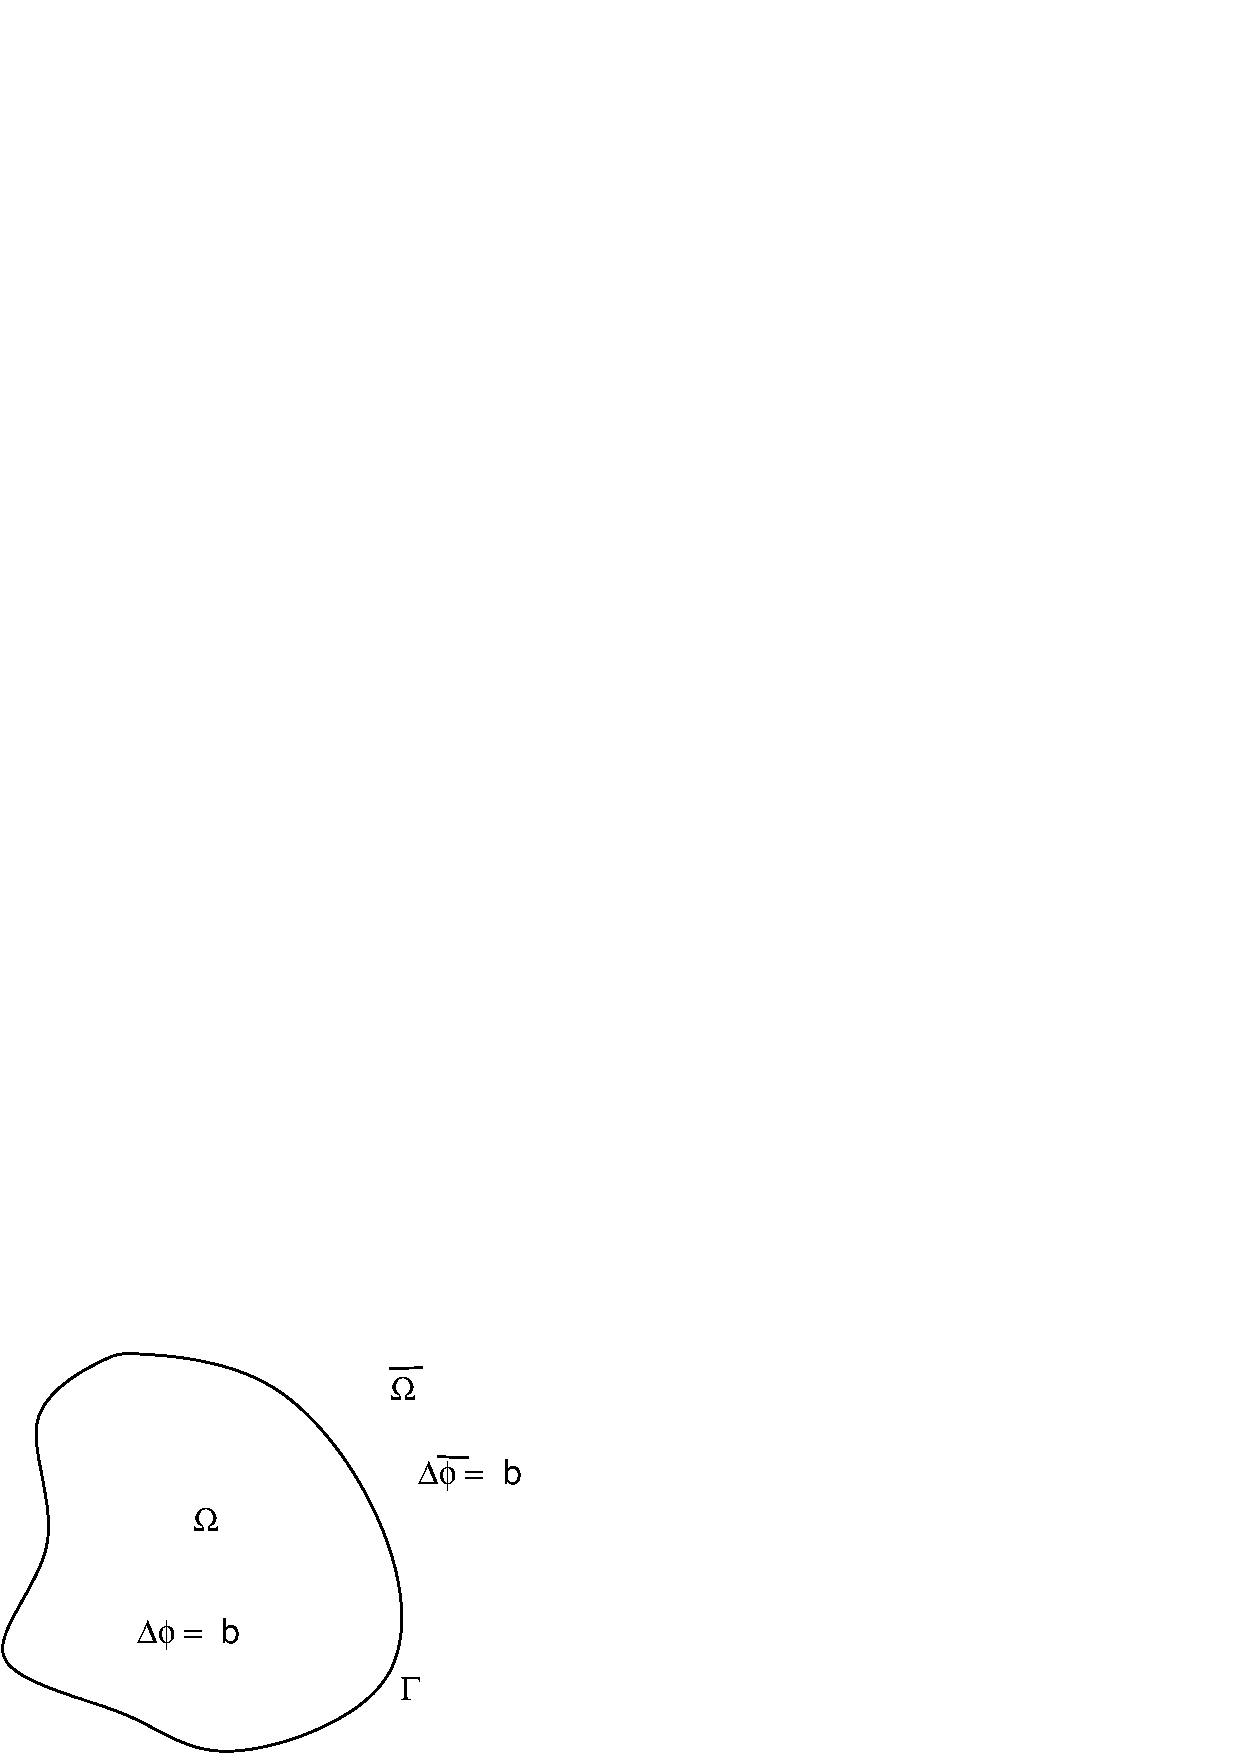
\includegraphics[width=0.4\textwidth]{ibem_domain_poisson.pdf}
\end{center}
\caption{The Poisson problem domain for the definition of the IBEM equations.}
\label{ibem_poisson_fig}
\end{figure}

In this case the equation that must be obeyed by the potential at any point in the domain $\Omega$ is given by:

\begin{equation}c(\vec{r})\phi(\vec{r})+\int_\Gamma{\phi(\vec{r}^\prime)H(\vec{r},\vec{r}^\prime)d\Gamma^\prime}=\int_\Gamma{q(\vec{r}^\prime)G(\vec{r},\vec{r}^\prime)d\Gamma^\prime}-\int_\Omega{b(\vec{r}^\prime)G(\vec{r},\vec{r}^\prime)d\Omega^\prime}\label{dbem_poisson_in}\end{equation}

For the complementary domain we have a similar expression:

\begin{equation}\overline{c}(\vec{r})\overline{\phi}(\vec{r})+\int_\Gamma{\overline{\phi}(\vec{r}^\prime)H(\vec{r},\vec{r}^\prime)d\Gamma^\prime}=\int_\Gamma{\overline{q}(\vec{r}^\prime)G(\vec{r},\vec{r}^\prime)d\Gamma^\prime}-\int_{\overline{\Omega}}{b(\vec{r}^\prime)G(\vec{r},\vec{r}^\prime)d\Omega^\prime}\label{dbem_poisson_out}\end{equation}

Just like inthe previous section, for any point at position $\vec{r}$ interior to $\Omega$ we have $c(\vec{r})=1$ and $\overline{c}(\vec{r})=0$, so we can re-write equations (\ref{dbem_poisson_in}) and (\ref{dbem_poisson_out}) as:

\begin{eqnarray}\phi(\vec{r})&+&\int_\Gamma{\phi(\vec{r}^\prime)H(\vec{r},\vec{r}^\prime)d\Gamma^\prime}=\int_\Gamma{q(\vec{r}^\prime)G(\vec{r},\vec{r}^\prime)d\Gamma^\prime}-\int_\Omega{b(\vec{r}^\prime)G(\vec{r},\vec{r}^\prime)d\Omega^\prime}\\&&\int_\Gamma{\overline{\phi}(\vec{r}^\prime)H(\vec{r},\vec{r}^\prime)d\Gamma^\prime}=\int_\Gamma{\overline{q}(\vec{r}^\prime)G(\vec{r},\vec{r}^\prime)d\Gamma^\prime}-\int_{\overline{\Omega}}{b(\vec{r}^\prime)G(\vec{r},\vec{r}^\prime)d\Omega^\prime}\end{eqnarray}

Preceeding as in section \ref{sec_laplace} we add these two equations, and using both in $q$ and $\overline{q}$ the normal exterior to $\Omega$, we obtain the following expression:

\begin{equation}\phi(\vec{r})+\int_\Gamma{\left[\phi(\vec{r}^\prime)-\overline{\phi}(\vec{r}^\prime)\right]H(\vec{r},\vec{r}^\prime)d\Gamma^\prime}=\int_\Gamma{\left[q(\vec{r}^\prime)+\overline{q}(\vec{r}^\prime)\right]G(\vec{r},\vec{r}^\prime)d\Gamma^\prime}-\int_{\Omega+\overline{\Omega}}{b(\vec{r}^\prime)G(\vec{r},\vec{r}^\prime)d\Omega^\prime}\end{equation}

Using the definitions (\ref{source_density}) and (\ref{dipole_density}) we can re-write this expression with a source term and a dipole term:

\begin{equation}\phi(\vec{r})=\int_\Gamma{m(\vec{r}^\prime)H(\vec{r},\vec{r}^\prime)d\Gamma^\prime}+\int_\Gamma{s(\vec{r}^\prime)G(\vec{r},\vec{r}^\prime)d\Gamma^\prime}-\int_{\Omega+\overline{\Omega}}{b(\vec{r}^\prime)G(\vec{r},\vec{r}^\prime)d\Omega^\prime}\label{ibem_poisson}\end{equation}

As expected, this expression is very similar to the one obtained in the case of Laplace equation, with the exception of the domain integral due to the body force term.
\pagebreak

\part{Implementation Details}
\pagebreak
\section*{}
\pagebreak

\chapter{Element Library}
We have used the following convention for the nodes in the elements:

\begin{figure}[!hbt]
\begin{minipage}[b]{0.5\linewidth}
\centering
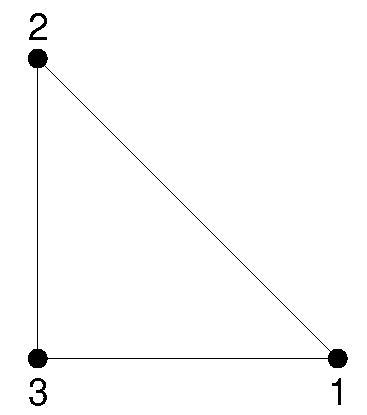
\includegraphics[width = 0.4\linewidth]{tria3.pdf}
\caption{Linear interpolation.}
\end{minipage}
\hspace{0.5cm}
\begin{minipage}[b]{0.5\linewidth}
\centering
\includegraphics[width = 0.4\linewidth]{tria6.pdf}
\caption{Quadratic interpolation.}
\end{minipage}
\end{figure}

Using this convention the shape functions for the linear case are simply given by:

\begin{eqnarray}
N_1 & = & L_1 \\
N_2 & = & L_2 \\
N_3 & = & 1-L_1-L_2
\end{eqnarray}

Under this convention the quadratic interpolation shape functions are given by:

\begin{eqnarray}
N_1 & = & L_1(2L_1-1) \\
N_2 & = & 4L_1L_2 \\
N_3 & = & L_2(2L_2-1) \\
N_4 & = & 4L2(1-L_1-L_2) \\
N_5 & = & L_3[1-2(L_1+L_2)] \\
N_6 & = & 4L_1(1-L_1-L_2)\end{eqnarray}

\pagebreak

\chapter{Numerical Integration}

\section{Regular integrals}
For non-singular integrals the integration is done using gaussian quadrature with NG integration points per element as in:

\begin{equation}
\int_{-1}^1{F(L_1,L_2)dL_1dL_2} \approx \sum_{i=1}^{NG}{F(L_1^i,L_2^i)w_i}
\end{equation}

By default the program uses 7 points per triangular element. Tests where done with 16 and 64 points per element and the accuracy of the results was not affected, so 7 points were kept for speed.

\section{Weakly singular integrals}
For weakly singular integrals the integration is done through a regularization transformation that eliminates the singularity. The element is transformed into a triangle with a singularity in node 1 and then into a degenerate square. In the degenerate square we can use Gauss-Jacobi integration to integrate getting rid of the singularity. See Figure \ref{fig:weak3} for the transformation.

\begin{equation}
\int_{-1}^1{F(L_1,L_2)(1+L_2)dL_1dL_2} \approx \sum_{i=1}^{NG}{\sum_{j=1}^{NG}{F(L_1^i,L_2^j)w_i^{\rm Gauss}w_j^{\rm Gauss-Jacobi}}}
\end{equation}

Notice that the Gauss-Jacobi integration is necessary in only one of the directions, so in the other the standard Gauss quadrature on a line is used and the product of the two provides the correct integration as indicated by the expression above.

\begin{figure}[!hbt]
\begin{center}
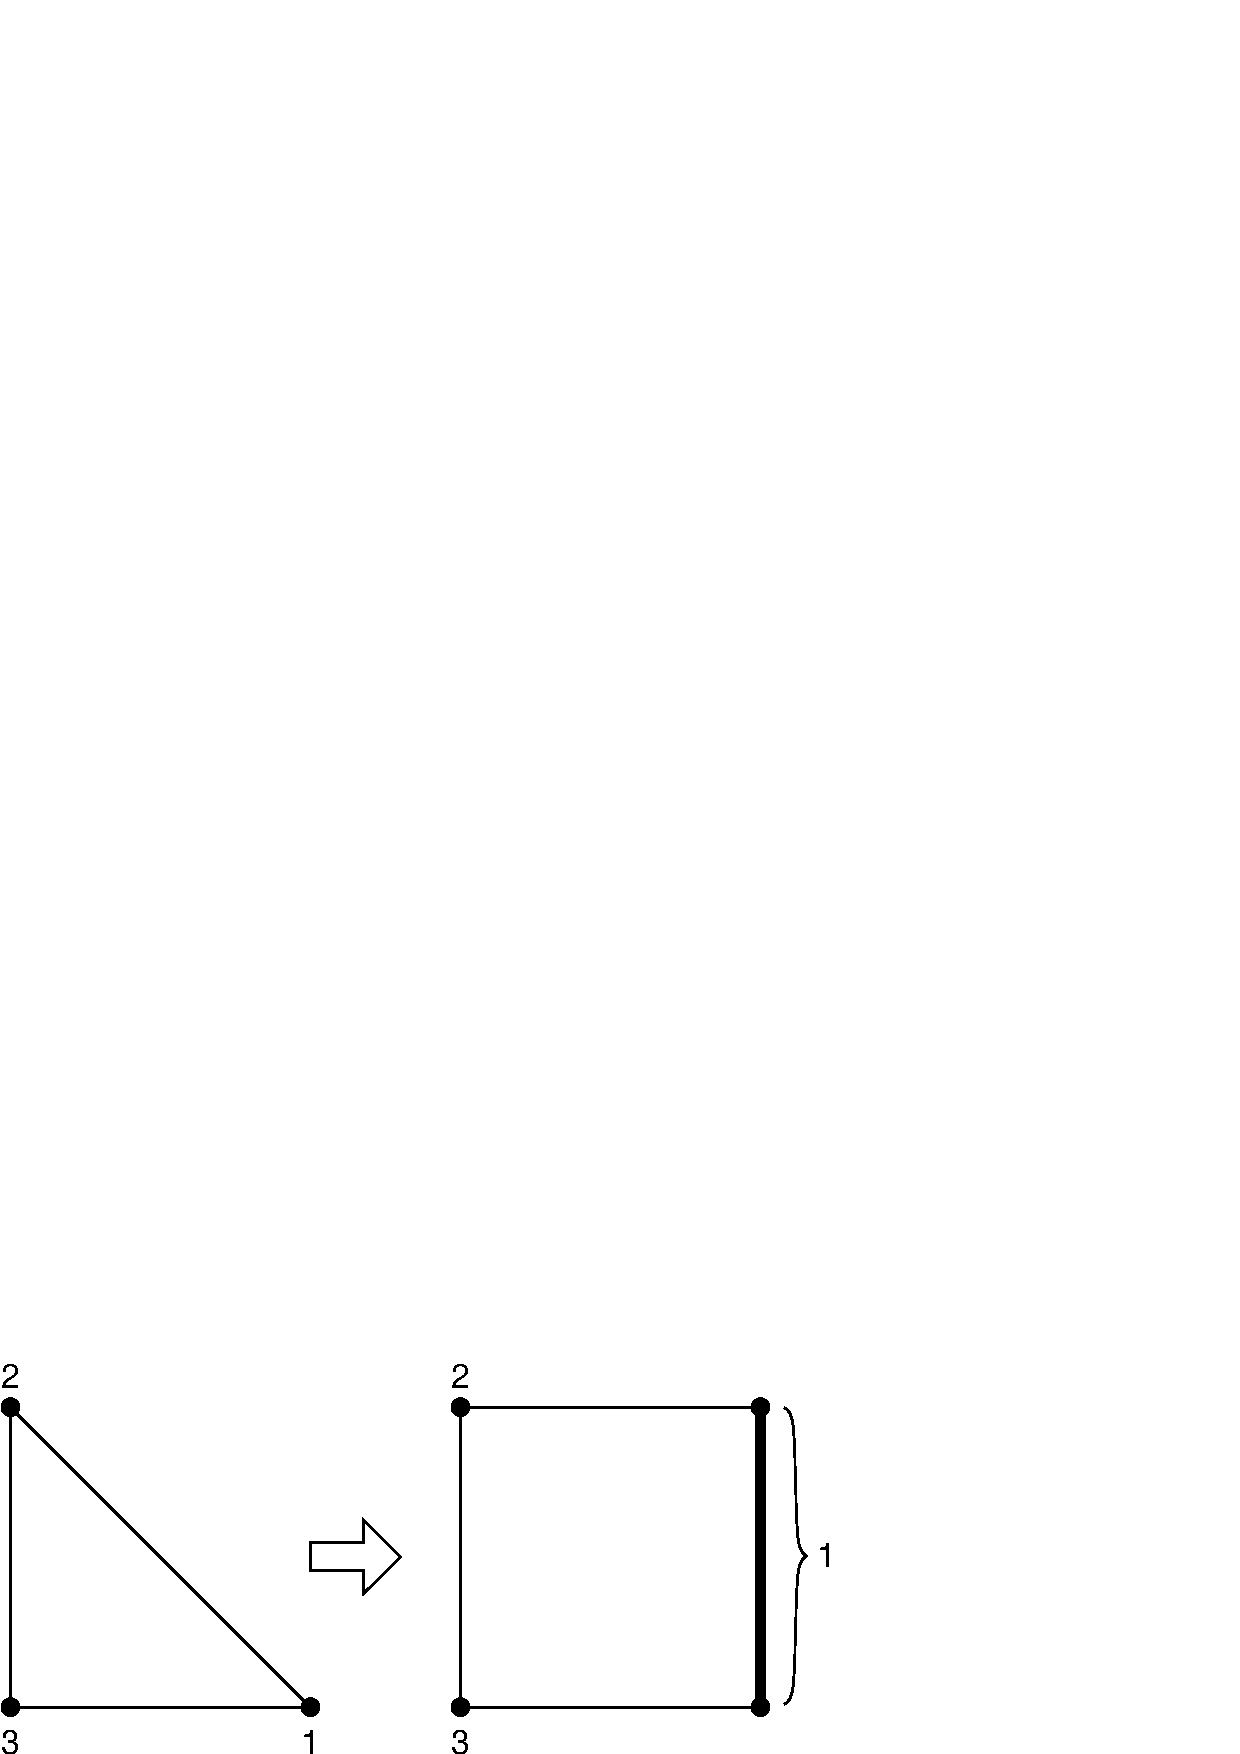
\includegraphics[width=0.6\textwidth]{weakly_singular.pdf}
\caption{Regularization transformation for weakly singular integrals (linear case).}
\label{fig:weak3}
\end{center}
\end{figure}

In the case of quadratic triangles when the singular point is on an edge of the triangle rather than on a vertex the triangle is divided in two and then the same regularization procedure is applied to both subtriangles as shown in Figure \ref{fig:weak6}.

\begin{figure}[!hbt]
\begin{center}
\includegraphics[width=\textwidth]{weakly_singular_t6.pdf}
\caption{Regularization transformation for weakly singular integrals (quadratic case).}
\label{fig:weak6}
\end{center}
\end{figure}

\section{Strongly singular integrals}
For strongly singular integrals we subdivide the triangle progressively in up to \verb+NSUBDIVISIONS+ --found in file \verb+constants.h+-- subsequent divisions, and integrate using standard gausian quadrature in each subtriangle except the closest to the singular point, which is neglected (it can be shown that the integrand goes to zero very close to the singularity point). The subdivision process is ilustrated in Figure \ref{fig:strong} for a singularity at node 3 in a flat triangle.

\begin{figure}[!hbt]
\begin{center}
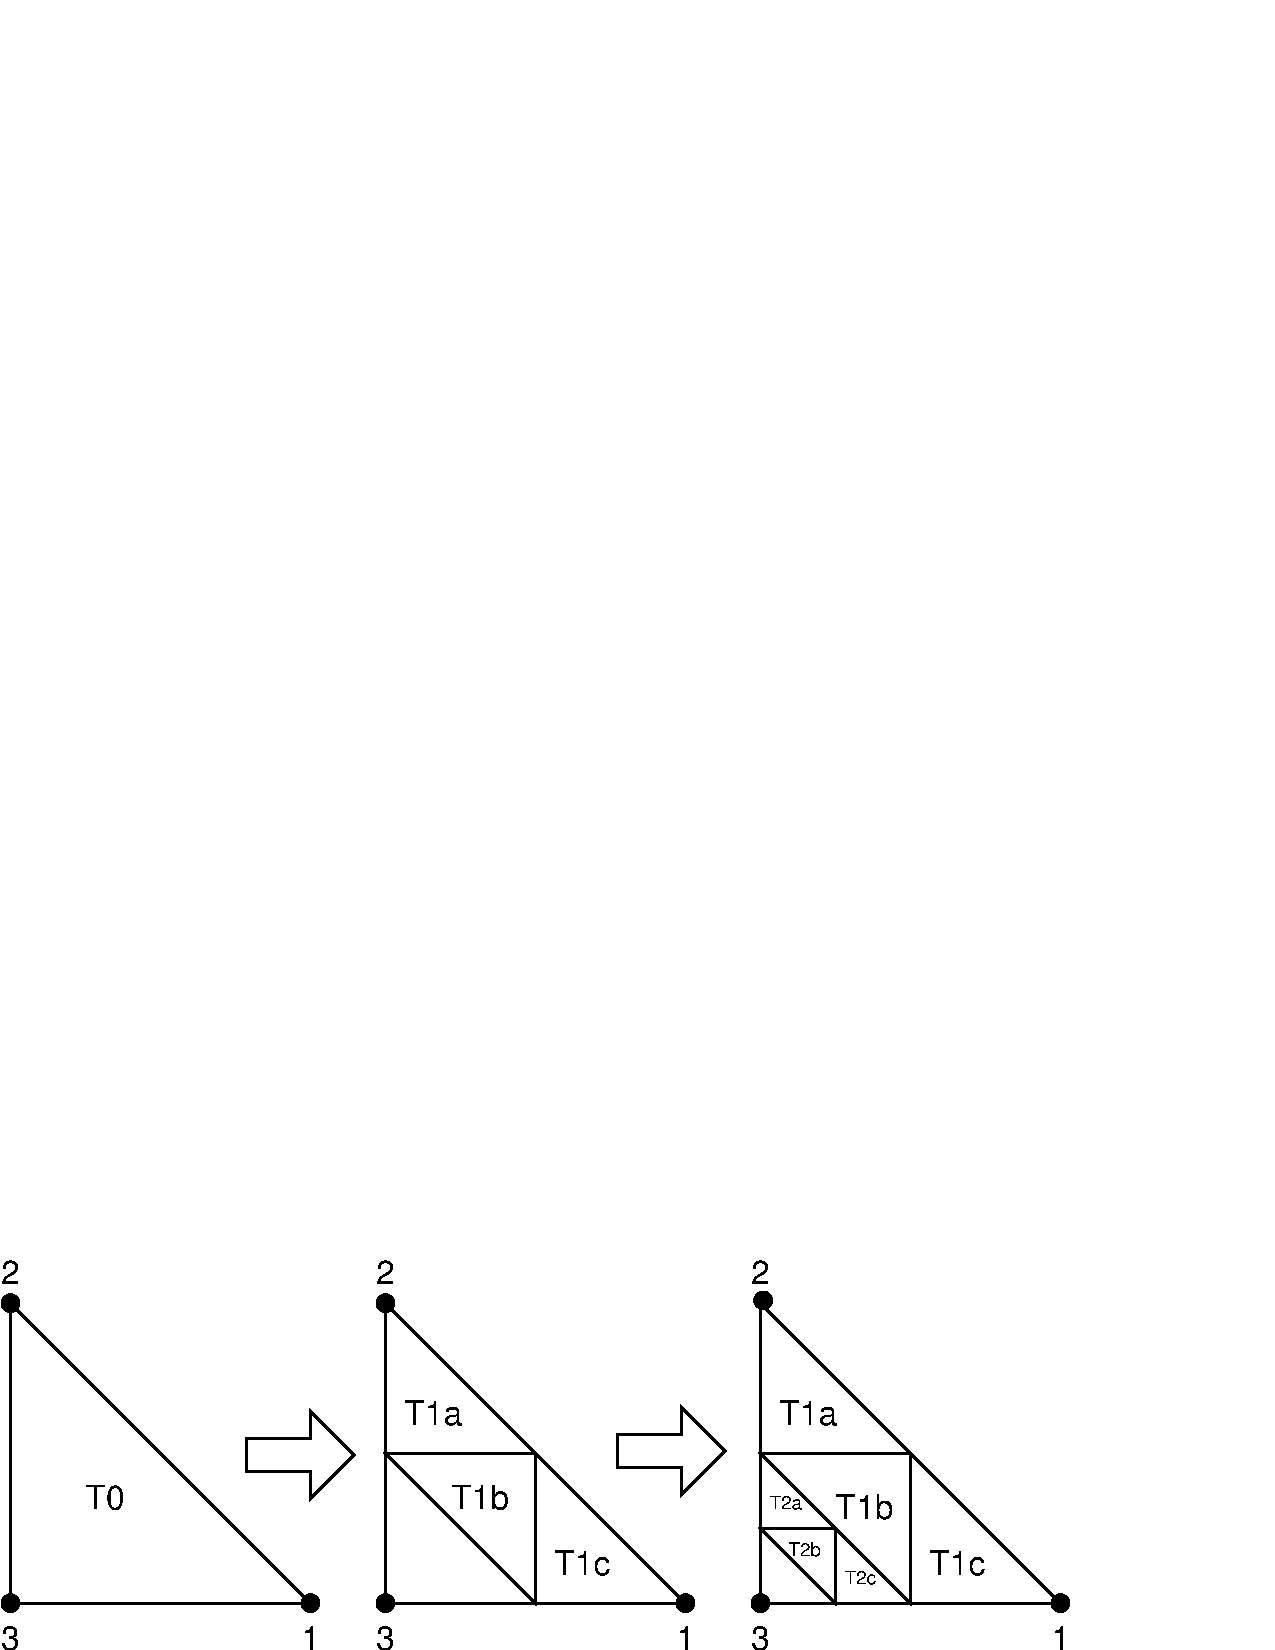
\includegraphics[width=0.9\textwidth]{strongly_singular.pdf}
\caption{Subdivision process for strongly singular integrands with singularity at node 3 (only two consecutive subdivisions shown).}\label{fig:strong}
\end{center}
\end{figure}

In the cases where the singular point is on the edge of a quadratic element rather than on a vertex the triangle is divided in two and the same subdivision process applied to the resulting subtriangles.

\section{Changing the number of integration points}
The gaussian quadrature data is stored in the file \verb+gaussData.h+, and has two options, one with 7 integration points and another one with 64 integrations points. By default the code uses 7 integration points because increasing this number does not seem to improve accuracy, but this can be changed by following these steps:

\begin{enumerate}
\item Change the value of \verb+TNGAUSS+ and \verb+TSNGAUSS+ to 64 in file \verb+constants.h+
\item Comment out the 7 point \verb+TGauss+ and \verb+TSGauss+ matrices in file \verb+gaussData.h+
\item Uncomment the 64 point \verb+TGauss+ and \verb+TSGauss+ matrices in file \verb+gaussData.h+
\item Recompile the source code
\end{enumerate}

The constant values \verb+TNGAUSS+ and \verb+TSNGAUSS+ are the number of integration points in regular and strongly singular integrals, so it is also possible to use different values for them. Keep in mind that \verb+NSUBDIVISIONS+ are made in the case of strongly singular integrals, and therefore many more points are used for the integration even if \verb+TNGAUSS+ and \verb+TSNGAUSS+ are given the same value.

All integration schemes were chosen so that the integration points are in the interior of the elements, avoiding issues with evaluation points falling exactly on top of mesh nodes. The numerical values of the gaussian integration are reproduced in the following tables.

\pagebreak
\begin{center}
\begin{tabular}{|c|c|c|c|}
\multicolumn{4}{c}{Table 1: Abscissas and weights for Gauss quadrature on a triangle}\\
\hline
NG & $x_i$ & $y_i$ & $w_i$\\
\hline\hline
7 & 0.333333333333333 & 0.333333333333333 & 0.112500000000000\\
 & 0.470142064105115 & 0.470142064105115 & 0.066197076394253\\
 & 0.059715871789770 & 0.470142064105115 & 0.066197076394253\\
 & 0.470142064105115 & 0.059715871789770 & 0.066197076394253\\
 & 0.101286507323456 & 0.101286507323456 & 0.062969590272414\\
 & 0.797426985353088 & 0.101286507323456 & 0.062969590272414\\
 & 0.101286507323456 & 0.797426985353088 & 0.062969590272414\\
\hline
\end{tabular}
\end{center}

\begin{center}
\begin{tabular}{|c|c|c|}
\multicolumn{3}{c}{Table 2: Abscissas and weights for Gauss-Jacobi quadrature on a line}\\
\hline
NG & $x_i$ & $w_i$\\
\hline\hline
8 & -0.910732089420060 & 0.013180765768995\\
 & -0.711267485915709 & 0.713716106239446\\
 & -0.426350485711139 & 0.181757278018796\\
 & -0.090373369606853 & 0.316798397969277\\
 & 0.256135670833455 & 0.424189437743720\\
 & 0.571383041208738 & 0.450023197883551\\
 & 0.817352784200412 & 0.364476094545495\\
 & 0.964440169705273 & 0.178203217446225\\
\hline
\end{tabular}
\end{center}

\begin{center}
\begin{tabular}{|c|c|c|}
\multicolumn{3}{c}{Table 3: Abscissas and weights for Gauss quadrature on a line}\\
\hline
NG & $x_i$ & $w_i$\\
\hline\hline
8 & -0.960289856497536 & 0.101228536290370\\
 & -0.796666477413627 & 0.222381034453376\\
 & -0.525532409916329 & 0.313706645877887\\
 & -0.183434642495650 & 0.362683783378362\\
 & 0.183434642495650 & 0.362683783378362\\
 & 0.525532409916329 & 0.313706645877887\\
 & 0.796666477413627 & 0.222381034453376\\
 & 0.960289856497536 & 0.101228536290370\\
\hline
\end{tabular}
\end{center}

\pagebreak
\section*{}
\pagebreak
\chapter{The electrostatic problem in DEP traps}\label{sec_electrostatic}
This chapter describes in detail the equations used by \verb+depSolver+ to calculate the electric field and the forces acting in dielectrophoretic traps -- the original application \verb+depSolver+ was written for.

Dielectrophoretic traps work by exerting a force on a particle due to the interaction of the polarization field in the particle with the gradient of the applied field \cite{Jones1995}. A detailed knowledge of the electric field on the surface of the particle is necessary in order to calculate the total force that it experiences at any given moment in time.

This problem consists in a flow chamber that has a certain set of electrodes on the bottom and the ceiling of the channel, forming a dielectrophoretic trap. The chamber encloses a liquid and several particles with different electrical properties, as shown in Figure \ref{fig:laplace_domain}.

\begin{figure}[hbt]
\begin{center}
\includegraphics[width=0.6\textwidth]{ibem_laplace.pdf}
\end{center}
\caption{Laplace problem with different materials. Note definition of normal vectors.}\label{fig:laplace_domain}
\end{figure}

A fixed (in DC) or alternating (in AC) potential is applied on the electrodes and we are interested in the potential and electric field inside the trap volume. The boundary conditions are continuity of the potential and the normal component of the electric displacement across dielectric boundaries and the given potential at the electrodes. Due to the absence of sources inside the volume (the particles are supposed to be neutral) we only need to solve Laplace's equation in each subdomain and match the boundary conditions at all surfaces.

In order to solve the problem we use the indirect boundary element method. To do this we discretize the system surfaces into elements and then apply the equations obtained in the following sections to get a linear system of equations. The advantage of the indirect method over the direct one is that we need only to apply a single equation on each node in the surface mesh.

\section{IBEM treatment of the electrostatic problem}\label{sec_ibem_electrostatic}
As mentioned above, Laplace equation must be must be satisfied in all subdomains (that is, inside each cell as well as in the liquid itself), and the potential and the normal derivative of the electric displacement must be continuous across all dielectric interfaces.

Because of the continuity of the electric potential we have to make the term $m(\vec{r}^\prime)$ equal to zero, and thus we can use equation (\ref{ibem_source_final}):

\begin{equation}
\phi(\vec{r})=\int_\Gamma{s(\vec{r}^\prime)G(\vec{r},\vec{r}^\prime)d\Gamma^\prime}\label{ibem_source}
\end{equation}

Where $\Gamma$ represents the total surface of the system, given by:

\begin{equation}
\Gamma=\Gamma_{\rm{e}}+\sum_{i=1}^{Np}\Gamma_i
\end{equation}
 
In electrostatics the normal derivatives of the potential correspond to the normal components of the electric field, so the source $s(\vec{r})$ can be written as:

\begin{equation}
s(\vec{r})=q(\vec{r}^\prime)+\overline{q}(\vec{r}^\prime)=E_{\rm n}(\vec{r}^\prime)-\overline{E}_{\rm n}(\vec{r}^\prime)
\end{equation}

Using Gauss' Law jump condition we can write:

\begin{equation}
s(\vec{r})=E_{\rm n}(\vec{r}^\prime)-\overline{E}_{\rm n}(\vec{r}^\prime)=\frac{\rho_{\rm s}(\vec{r}^\prime)}{\varepsilon_0}
\end{equation}

where $\varepsilon_0$ is the permittivity of free space and $\rho_{\rm s}$ is the total surface charge density in $\Gamma$. For convenience we will redefine G and H as:

\begin{eqnarray}
G^{3D}(\vec{r},\vec{r}^\prime)&=&\frac{1}{r}\label{green}\\
H^{3D}(\vec{r},\vec{r}^\prime)&=&-\frac{(\vec{r}-\vec{r}^\prime)\cdot\hat{n}}{|\vec{r}-\vec{r}^\prime|^3}
\end{eqnarray}

So that the correct expression for the potential results in:

\begin{equation}
\phi(x)=\frac{1}{4\pi\varepsilon_0}\int_\Gamma{\rho_{\rm s}(\vec{r}^\prime)G(\vec{r},\vec{r}^\prime)d\Gamma^\prime}\label{pot_electrostatic}
\end{equation}

\subsection{DC Case}\label{sec_dc}
In this case we consider lossless media, and the boundary conditions at the dielectric interfaces are given by:

\begin{eqnarray}\left.\phi_{\rm{e}}\right|_{\Gamma_{\rm{i}}}&=&\left.\phi_{\rm{i}}\right|_{\Gamma_{\rm{i}}}\label{pot_continuity}\\\varepsilon_{\rm{e}}\left.\frac{\partial\phi_{\rm{e}}}{\partial n}\right|_{\Gamma_{\rm{i}}}&=&\varepsilon_{\rm{i}}\left.\frac{\partial\phi_{\rm{i}}}{\partial n}\right|_{\Gamma_{\rm{i}}}\label{pot_deriv_continuity}\end{eqnarray}

for all dielectric interfaces i.

Taking the derivative of (\ref{pot_electrostatic}) at a point not in the surface gives:

\begin{equation}\frac{\partial\phi(\vec{r})}{\partial n}=\frac{1}{2\alpha\pi\varepsilon_0}\int_\Gamma{\rho_{\rm s}(\vec{r}^\prime)H(\vec{r},\vec{r}^\prime)d\Gamma^\prime}\end{equation}

When taking this expression to the boundary we must include the jump in the integral due to the discontinuity of the normal derivative of the potential:

\begin{equation}\frac{\partial\phi_{\rm{e}}(\vec{r})}{\partial n}=-\frac{\rho_{\rm s}(\vec{r})}{2\varepsilon_0}+\frac{1}{2\alpha\pi\varepsilon_0}\int_\Gamma{\rho_{\rm s}(\vec{r}^\prime)H(\vec{r},\vec{r}^\prime)d\Gamma^\prime}\qquad\textrm{if $\vec{r}\in\Gamma_{\rm{i}}$}\end{equation}

\begin{equation}\frac{\partial\phi_{\rm{i}}(\vec{r})}{\partial n}=\frac{\rho_{\rm s}(\vec{r})}{2\varepsilon_0}+\frac{1}{2\alpha\pi\varepsilon_0}\int_\Gamma{\rho_{\rm s}(\vec{r}^\prime)H(\vec{r},\vec{r}^\prime)d\Gamma^\prime}\qquad\textrm{if $\vec{r}\in\Gamma_{\rm{i}}$}\end{equation}

Using these expression in the boundary condition (\ref{pot_deriv_continuity}) gives:

\begin{equation}\varepsilon_{\rm{e}}\left[-\frac{\rho_{\rm s}(\vec{r})}{2\varepsilon_0}+\frac{1}{2\alpha\pi\varepsilon_0}\int_\Gamma{\rho_{\rm s}(\vec{r}^\prime)H(\vec{r},\vec{r}^\prime)d\Gamma^\prime}\right]=\varepsilon_{\rm{i}}\left[\frac{\rho_{\rm s}(\vec{r})}{2\varepsilon_0}+\frac{1}{2\alpha\pi\varepsilon_0}\int_\Gamma{s(\vec{r}^\prime)H(\vec{r},\vec{r}^\prime)d\Gamma^\prime}\right]\end{equation}

Reorganizing terms to isolate the integrals to the right we get:

\begin{equation}
-\frac{(\varepsilon_{\rm{i}}+\varepsilon_{\rm{e}})\rho_{\rm s}(\vec{r})}{2\varepsilon_0}=\frac{(\varepsilon_{\rm{i}}-\varepsilon_{\rm{e}})}{2\alpha\pi\varepsilon_0}\int_\Gamma{\rho_{\rm s}(\vec{r}^\prime)H(\vec{r},\vec{r}^\prime)d\Gamma^\prime}
\end{equation}

And finally, for any point in the boundary $\Gamma_{\rm{i}}$ we find:

\begin{equation}
\rho_{\rm s}(\vec{r})=\frac{\varepsilon_{\rm{e}}-\varepsilon_{\rm{i}}}{\alpha\pi(\varepsilon_{\rm{e}}+\varepsilon_{\rm{i}})}\int_\Gamma{\rho_{\rm s}(\vec{r}^\prime)H(\vec{r},\vec{r}^\prime)d\Gamma^\prime}\label{source_electrostatic}
\end{equation}

So using (\ref{pot_electrostatic}) evaluated on te external boundary, and (\ref{source_electrostatic}) on each of the internal boundaries we can solve for $\sigma$, and then calculate the potential from (\ref{pot_electrostatic}) at any point in the domain. Any derivative of the potential can be calcualted by taking the derivative in (\ref{pot_electrostatic}), which will affect only $x$ and therefore leave the $\sigma$ as constants.

\subsection{AC case}
When real materials are studied the losses have to be included in the calculations, so we must consider not only the dielectric permittivity but also the electric conductivity of the material. It is also the case that the electrical response of the material will appear to have a time lag with respect to the externally applied field. In the case of harmonic applied fields (periodic in time) this time lag is easily expressed as a phase difference between the applied field and the resulting current and polarization. A good reference for this problem is the work by Pohl \cite{Pohl1978} that we follow in this section.

For a simple (linear) medium if the applied field is harmonic, the charge density, current, polarization, and other descriptive electromagnetic parameters will also be harmonic, but not necessarily in phase with the applied field. If the applied field is given by:

\begin{equation}\vec{E}(\vec{r},t)=\vec{E}_0(\vec{r})\exp(j\omega t)\end{equation}

The we also have:

\begin{eqnarray}\vec{J}(\vec{r},t)&=&\vec{J}_0(\vec{r},t)\exp(j\omega t-j\delta_{\rm{J}})\\\vec{D}(\vec{r},t)&=&\vec{D}_0(\vec{r},t)\exp(j\omega t-j\delta_{\rm{D}})\\\vec{P}(\vec{r},t)&=&\vec{P}_0(\vec{r},t)\exp(j\omega t-j\delta_{\rm{P}})\\\rho(\vec{r},t)&=&\rho_0(\vec{r},t)\exp(j\omega t-j\delta_\rho)\\\vec{B}(\vec{r},t)&=&\vec{B}_0(\vec{r},t)\exp(j\omega t-j\delta_{\rm{B}})\\\vec{H}(\vec{r},t)&=&\vec{H}_0(\vec{r},t)\exp(j\omega t-j\delta_{\rm{H}})\end{eqnarray}

And for homogeneous, isotropic media we can write:

\begin{eqnarray}
\vec{D}&=&\varepsilon\vec{E}\label{electric_displacement}\\
\vec{J}&=&\sigma\vec{E}\label{electric_current}
\end{eqnarray}

Where both $\varepsilon$ and $\sigma$ are complex quantities. Maxwell's equations are given by:

\begin{eqnarray}
\nabla\vec{E}&=&\frac{\rho}{\varepsilon}\\\nabla\times\vec{E}&=&-\frac{\partial\vec{B}}{\partial t}\\
\nabla\cdot\vec{B}&=&0\\\nabla\times\vec{H}&=&\vec{J}+\frac{\partial\vec{D}}{\partial t}
\end{eqnarray}

which in this case, and using (\ref{electric_displacement}) and (\ref{electric_current}) reduce to:

\begin{eqnarray}
\nabla\vec{E}&=&\frac{\rho}{\varepsilon}\label{divE}\\\nabla\times\vec{E}&=&-j\omega\vec{B}\\
\nabla\cdot\vec{B}&=&0\\\nabla\times\vec{H}&=&\left[\sigma+i\omega\varepsilon\right]\vec{E}
\end{eqnarray}

Now, the boundary conditions at a dielectric interface between materials 1 and 2 are given by:

\begin{eqnarray}
\varepsilon_1E_{1\rm{n}}-\varepsilon_2E_{2\rm{n}}&=&-\rho_{\rm{free}}\\
\left(\hat{n}\times\vec{E}_1\right)-\left(\hat{n}\times\vec{E}_2\right)&=&0\\
\left(\hat{n}\times\vec{H}_1\right)-\left(\hat{n}\times\vec{H}_2\right)&=&-\vec{I}_{\rm{free}}\\B_{1\rm{n}}-B_{2\rm{n}}&=&0
\end{eqnarray}

with $\rho_{\rm free}$ the surface density of free charge, and $\vec{I}_{\rm free}$ the surface density of free current, which is different from zero only in perfect conductors.

The equations for the conservation of charge in a harmonic field are:

\begin{eqnarray}\varepsilon\nabla\vec{E}+j\omega\rho_{\rm free}&=&0\label{charge_conservation}\\\nabla\cdot\vec{I}_{\rm free}+j\omega\rho_{\rm free}-\hat{n}\cdot\left(\sigma_1\vec{E}_1-\sigma_2\vec{E}_2\right)&=& 0\label{flux_conservation}\end{eqnarray}

Using (\ref{divE}) into (\ref{charge_conservation}) we get:

\begin{equation}\nabla\left[(\varepsilon-i\sigma/\omega)\vec{E}\right]=0\end{equation}

everywhere except at the boundaries, where $\nabla(\varepsilon-i\sigma/\omega)\neq0$. Combining now (\ref{electric_current}) and (\ref{flux_conservation}) for a dielectric material ($I_{\rm free}=0$):

\begin{equation}(\varepsilon_1-j\sigma_1/\omega)E_{1\rm n}=(\varepsilon_2-j\sigma_2/\omega)E_{2\rm n}\end{equation}

If we define now the {\it complex permittivity} of a material as $\tilde{\varepsilon}=\varepsilon-j\sigma/\omega$, we can re-write the previous equations in terms of the potential:

\begin{equation}\nabla\left(\tilde{\varepsilon}\vec{E}\right)=\nabla^2\phi=0\end{equation}
\begin{equation}\tilde{\varepsilon}_1\frac{\partial\phi_1}{\partial n}=\tilde{\varepsilon}_2\frac{\partial\phi_2}{\partial n}\end{equation}

These are exactly the same equations that we used for the DC case, with the only difference that now both the permittivity and the potential are complex quantitites.

Call the total surface charge density $\rho_{\rm s}(\vec{r})$ the equations to solve in the indirect boundary element method are:

\begin{eqnarray}
\phi(\vec{r})&=&\frac{1}{2\alpha\pi\varepsilon_0}\int_\Gamma{\rho_{\rm s}(\vec{r}^\prime)G(\vec{r},\vec{r}^\prime)d\Gamma^\prime}\qquad\qquad\textrm{for a conductor}\label{ac_pot}\\
\rho_{\rm s}(\vec{r})&=&\frac{(\tilde{\varepsilon}_{\rm e}-\tilde{\varepsilon}_{\rm i})}{\alpha\pi(\tilde{\varepsilon}_{\rm e}+\tilde{\varepsilon}_{\rm i})}\int_\Gamma{\rho_{\rm s}(\vec{r}^\prime)H(\vec{r},\vec{r}^\prime)d\Gamma^\prime}\qquad\textrm{for a dielectric interface}\label{ac_source}\end{eqnarray}

with the boundary conditions:

\begin{eqnarray}
\left.\phi_{\rm e}\right|_{\Gamma_{\rm i}}&=&\left.\phi_{\rm i}\right|_{\Gamma_{\rm i}}\label{ac_bc1}\\
\tilde{\varepsilon}_{\rm e}\left.\frac{\partial\phi_{\rm e}}{\partial n}\right|_{\Gamma_{\rm i}}&=&\tilde{\varepsilon}_{\rm i}\left.\frac{\partial\phi_{\rm i}}{\partial n}\right|_{\Gamma_{\rm i}}\label{ac_bc2}
\end{eqnarray}

Expanding $\tilde{\varepsilon}$ in equation (\ref{ac_source}):

\begin{equation}
\rho_{\rm s}(\vec{r})=\frac{[(\sigma_{\rm e}+j\omega\varepsilon_{\rm e})-(\sigma_{\rm i}+j\omega\varepsilon_{\rm i})]}{\alpha\pi[(\sigma_{\rm e}+j\omega\varepsilon_{\rm e})-(\sigma_{\rm i}+j\omega\varepsilon_{\rm i})]}\int_\Gamma{\rho_{\rm s}(\vec{r}^\prime)G(\vec{r},\vec{r}^\prime)d\Gamma^\prime}
\end{equation}

which can be re-written as:

\begin{equation}
\rho_{\rm s}(\vec{r})=\frac{[(\sigma_{\rm e}-\sigma_{\rm i})+j\omega(\varepsilon_{\rm e}-\varepsilon_{\rm i})]}{\alpha\pi[(\sigma_{\rm e}+\sigma_{\rm i})+j\omega(\varepsilon_{\rm e}+\varepsilon_{\rm i})]}\int_\Gamma{\rho_{\rm s}(\vec{r}^\prime)G(\vec{r},\vec{r}^\prime)d\Gamma^\prime}
\end{equation}

Dividing now $\rho_{\rm s}(\vec{r})$ into its real and imaginary parts (denoted as $\rho_{\rm s}^{\rm R}(\vec{r})$ and $\rho_{\rm s}^{\rm I}(\vec{r})$ respectively) we get:

\begin{eqnarray}
&&\alpha\pi[\rho_{\rm s}^{\rm R}(\vec{r})+j\rho_{\rm s}^{\rm I}(\vec{r})][(\sigma_{\rm e}+\sigma_{\rm i})+j\omega(\varepsilon_{\rm e}+\varepsilon_{\rm i})]=\nonumber\\
&&[(\sigma_{\rm e}-\sigma_{\rm i})+j\omega(\varepsilon_{\rm e}-\varepsilon_{\rm i})]\int_\Gamma{[\rho_{\rm s}^{\rm R}(\vec{r}^\prime)+j\rho_{\rm s}^{\rm I}(\vec{r}^\prime)]H(\vec{r},\vec{r}^\prime)d\Gamma^\prime}
\end{eqnarray}

Separating all real and imaginary terms we obtain two equations:

\begin{eqnarray}
&&\alpha\pi[(\sigma_{\rm e}+\sigma_{\rm i})\rho_{\rm s}^{\rm R}(\vec{r})-\omega(\varepsilon_{\rm e}+\varepsilon_{\rm i})\rho_{\rm s}^{\rm I}(\vec{r})]=\nonumber\\
&&(\sigma_{\rm e}-\sigma_{\rm i})\int_\Gamma{\rho_{\rm s}^{\rm R}(\vec{r})H(\vec{r},\vec{r}^\prime)d\Gamma^\prime}-\omega(\varepsilon_{\rm e}-\varepsilon_{\rm i})\int_\Gamma{\rho_{\rm s}^{\rm I}(\vec{r})H(\vec{r},\vec{r}^\prime)d\Gamma^\prime}\label{sr}
\end{eqnarray}

\begin{eqnarray}
&&\alpha\pi[(\sigma_{\rm e}+\sigma_{\rm i})\rho_{\rm s}s^{\rm I}(\vec{r})+\omega(\varepsilon_{\rm e}+\varepsilon_{\rm i})\rho_{\rm s}^{\rm R}(\vec{r})]=\nonumber\\
&&\omega(\varepsilon_{\rm e}-\varepsilon_{\rm i})\int_\Gamma{\rho_{\rm s}^{\rm R}(\vec{r})H(\vec{r},\vec{r}^\prime)d\Gamma^\prime}+(\sigma_{\rm e}-\sigma_{\rm i})\int_\Gamma{\rho_{\rm s}^{\rm I}(\vec{r})H(\vec{r},\vec{r}^\prime)d\Gamma^\prime}\label{si}
\end{eqnarray}

We can isolate the real part of $\rho_{\rm s}(\vec{r})$ on the left by adding (\ref{sr})$\times(\sigma_{\rm e}+\sigma_{\rm i})$ and (\ref{si})$\times\omega(\varepsilon_{\rm e}+\varepsilon_{\rm i})$:

\begin{equation}
\rho_{\rm s}^{\rm R}(\vec{r})=A\int_\Gamma{\rho_{\rm s}^{\rm R}(\vec{r}^\prime)H(\vec{r},\vec{r}^\prime)d\Gamma^\prime}+B\int_\Gamma{\rho_{\rm s}^{\rm I}(\vec{r}^\prime)H(\vec{r},\vec{r}^\prime)d\Gamma^\prime}\label{sr_final}
\end{equation}

And we can isolate the imaginary part of $\rho_{\rm s}(x)$ on the left by subtracting (\ref{sr})$\times\omega(\varepsilon_{\rm e}+\varepsilon_{\rm i})$ from (\ref{si})$\times(\sigma_{\rm e}+\sigma_{\rm i})$:

\begin{equation}\rho_{\rm s}^{\rm I}(\vec{r})=A\int_\Gamma{s^{\rm I}(\vec{r}^\prime)H(\vec{r},\vec{r}^\prime)d\Gamma^\prime}-B\int_\Gamma{\rho_{\rm s}^{\rm R}(\vec{r}^\prime)H(\vec{r},\vec{r}^\prime)d\Gamma^\prime}\label{si_final}\end{equation}

Where the factors $A$ and $B$ are given by:

\begin{equation}A=\frac{(\sigma^2_{\rm e}-\sigma^2_{\rm i})+\omega^2(\varepsilon^2_{\rm e}-\varepsilon^2_{\rm i})}{\alpha\pi[(\sigma_{\rm e}+\sigma_{\rm i})^2+\omega^2(\varepsilon_{\rm e}+\varepsilon_{\rm i})^2]}\label{A}\end{equation}
\begin{equation}B=\frac{2\omega(\sigma_{\rm e}\varepsilon_{\rm i}-\sigma_{\rm i}\varepsilon_{\rm e})}{\alpha\pi[(\sigma_{\rm e}+\sigma_{\rm i})^2+\omega^2(\varepsilon_{\rm e}+\varepsilon_{\rm i})^2]}\label{B}\end{equation}

Equations (\ref{sr_final}--\ref{B}) are used in nodes situated in a dielectric boundary. For nodes in a conductor a simpler pair of equations is used:

\begin{equation}\phi^{\rm R}(\vec{r})=\frac{1}{2\alpha\pi\varepsilon_0}\int_\Gamma{\rho_{\rm s}^{\rm R}(\vec{r}^\prime)G(\vec{r},\vec{r}^\prime)d\Gamma^\prime}\end{equation}
\begin{equation}\phi^{\rm I}(\vec{r})=\frac{1}{2\alpha\pi\varepsilon_0}\int_\Gamma{\rho_{\rm s}^{\rm I}(\vec{r}^\prime)G(\vec{r},\vec{r}^\prime)d\Gamma^\prime}\end{equation}

NOTE: It is common to absorb $\varepsilon_0$ into $\rho_{\rm s}(\vec{r})$.

\section{Calculation of the DEP force}
This section describes the two alternative methods of calculating the electrical force in dielectrophoretic traps.

\subsection{Equivalent multipole model of the DEP force}
In this approach the particle under consideration is substituted by a series of multipoles that account for the local changes of the electric field in the region surrounding the particle \cite{Washizu1994},\cite{Jones1996}. This approximation is strictly valid only when the external field is not changing rapidly in the region containing the particle. 

\subsection*{Spherical particles}
In the simplest possible approximation, the time-averaged DEP force for a spherical particle is given by the expression:

\begin{equation}\left<\vec{F}_{\rm{DEP}}\right>=2\pi R^3\varepsilon_{\rm{f}}Re\left[K\left(\omega\right)\right]\nabla(E^2)\end{equation}

where $R$ is the particle radius, $\varepsilon_f$ is the permittivity of the fluid suspending medium, $E$ is the rms magnitude of the local electric field, and $Re[K(\omega)]$ is the real part of the Clausius-Mossotti factor, given by:

\begin{equation}K(\omega)=\frac{\tilde{\varepsilon}_{\rm{p}}-\tilde{\varepsilon}_{\rm{f}}}{\tilde{\varepsilon}_{\rm{p}}+2\tilde{\varepsilon}_{\rm{f}}}\end{equation}

where $\omega$ is the angular frequency of the external applied field and $\tilde{\varepsilon}_{\rm{f}}$ and $\tilde{\varepsilon}_{\rm{p}}$ are the complex dielectric permittivities of the fluid and the particle respectively. The complex permittivities are given by $\tilde{\varepsilon}_{\rm{i}}=\varepsilon_{\rm{i}}-j\sigma_{\rm{i}}/\omega$, where $\varepsilon_{\rm{i}}$ is the dielectric permittivity of medium i, $\sigma_{\rm{i}}$ is the electric conductivity of medium i, and $j$ is $\sqrt{-1}$. 

This is the dipolar approximation for the DEP force on a sphere, and it is used extensively in the literature to predict the characteristics of DEP cell traps.

The dipolar approximation is simple and convenient, but in cases where the electric field presents a null or a high gradient its results are not accurate. When designing single-cell traps the electric field gradient must be very high for the electric forces on the particle to be significant, and therefore a better approximation, including higher order multipolar terms, is needed.

The general expression of the DEP force in terms of its multipolar components obtained by Washizu and Jones [12,13] was recently extended to include the magnetic field effects by Washizu [17]. However, in the cases studied in the present work the magnetic effects are negligible, and the expression of the time averaged $n$th force order contribution is:

\begin{equation}\left<\vec{F}_{\rm{DEP}}^{(n)}\right>=\frac{1}{2}\frac{\mathbf{p}^{(n)}[\cdot]^n\left(\nabla\right)^n\vec{E}}{n!}\label{basic_mp_formula}\label{dep_order_n}\end{equation}

where $[\cdot]^n$ and $\left(\nabla\right)^n$ represent $n$ dot products and gradient operations, and $\mathbf{p}^{(n)}$ is the multipolar induced tensor of order $n$:

\begin{equation}\mathbf{p}^{(n)}=\frac{4\pi\varepsilon_{\rm{f}}R^{2n+1}n}{(2n+1)!!}K^{(n)}(\omega)\left(\nabla\right)^{n-1}\vec{E}\end{equation}

with $K^{(n)}$ the $n$th order Clausius-Mossotti factor given by:

\begin{equation}K^{(n)}(\omega)=\frac{\tilde{\varepsilon}_{\rm{p}}-\tilde{\varepsilon}_{\rm{f}}}{n\tilde{\varepsilon}_{\rm{p}}+(n+1)\tilde{\varepsilon}_{\rm{f}}}\end{equation}

Note that a factor $1/2$ is included in (\ref{dep_order_n}) in order to account for the time average, under the assumption that the external field oscillates harmonically.

A BEM calculation is used to find the external field produced by the electrode arrangement, and its derivatives, in order to find the force using this approximation. Once the field and its derivatives are calculated on the centre of the sphere, a simple application of the formulas above gives the total DEP force on the particle. 

\subsection*{Ellipsoidal particles}
The induced effective moment for an ellipsoidal particle with principal radii a, b, and c, can be found by examining the limit of the electrostatic potential at a point far from the ellipsoid, where ellipsoidal coordinates degenerate into spherical coordinates. Following Jones \cite{Jones1995} the x component of the effective dipole moment due to a dielectric ellipsoid is given by:

\begin{equation}\rm{p}_{\rm{x}}=\frac{4\pi abc}{3}\varepsilon_{\rm{f}}\left[\frac{\varepsilon_{\rm{p}}-\varepsilon_{\rm{f}}}{\varepsilon_{\rm{f}}+(\varepsilon_{\rm{p}}-\varepsilon_{\rm{f}})L_{\rm{x}}}\right]E_{\rm{x}}\end{equation}

The other two components of the effective moment, $\rm{p}_{\rm{y}}$ and $\rm{p}_{\rm{y}}$, are of similar form. The time-averaged dielectrophoretic force produced by a harmonically oscillating external field on the ellipsoid is then given by the following expression:

\begin{equation}\left<\vec{F}_{\rm{DEP}}^{\rm{ellipsoid}}\right>=\frac{2\pi abc}{3}\varepsilon_{\rm{f}}\left[\frac{(\varepsilon_{\rm{p}}-\varepsilon_{\rm{f}})E_{\rm{x}}\partial_{\rm{x}}}{\varepsilon_{\rm{f}}+(\varepsilon_{\rm{p}}-\varepsilon_{\rm{f}})L_{\rm{x}}}+\frac{(\varepsilon_{\rm{p}}-\varepsilon_{\rm{f}})E_{\rm{y}}\partial_{\rm{y}}}{\varepsilon_{\rm{f}}+(\varepsilon_{\rm{p}}-\varepsilon_{\rm{f}})L_{\rm{y}}}+\frac{(\varepsilon_{\rm{p}}-\varepsilon_{\rm{f}})E_{\rm{z}}\partial_{\rm{z}}}{\varepsilon_{\rm{f}}+(\varepsilon_{\rm{p}}-\varepsilon_{\rm{f}})L_{\rm{z}}}\right]\vec{E}\end{equation}

Where the depolarization factors $L_{\rm{x}}$, $L_{\rm{y}}$, and $L_{\rm{z}}$, are all positive and interrelated as follows:

\begin{eqnarray}&& 0\leq L_i\leq 1,\qquad i=x,y,z \\ && L_{\rm{x}}+L_{\rm{y}}+L_{\rm{z}}=1\end{eqnarray}

The value of $L_{\rm{x}}$ is given by an elliptic integral:

\begin{equation}L_{\rm{x}}=\frac{abc}{2}\int^\infty_0{\frac{ds}{(s+a^2)\sqrt{(s+a^2)(s+b^2)(s+c^2)}}}\end{equation}

Similar expressions apply for y and z by simply changing the $(s+a^2)$ outside the square root by $(s+b^2)$ or $(s+c^2)$.

Note that this is only a first order approximation and therefore it will predict zero force for any particle position such that the ellipsoid's centre corresponds to a field null.

\subsection{Maxwell stress tensor derivation of the DEP force}
A different approach to the calculation of the DEP force is to use the Maxwell stress tensor formulation and integrate the stress tensor $\mathbf{T}$ over the surface of the particle:

\begin{equation}\vec{F}(t)_{\rm{DEP}}^{\rm{MST}}=\oint{\left(\mathbf{T}\cdot\vec{n}\right)dA}\end{equation}

where $\vec{n}$ is the unit vector normal to the surface and $t$ is time. This is regarded as the most rigurous approach to derive field-induced forces.

The general expression for the DEP force obtained by Wang et al \cite{Wang1997} is used in order to find out how precise the multipolar approximation is when compared to this more rigurous calculation.

The time-averaged net DEP force on a particle using MST is given by:

\begin{equation}\left<\vec{F}_{\rm{DEP}}^{\rm{MST}}\right>=\frac{\varepsilon_{\rm{f}}}{4}\oint{\left\{\left[\left(\vec{E}_{\rm{f}}\vec{E}^*_{\rm{f}}+\vec{E}^*_{\rm{f}}\vec{E}_{\rm{f}}\right)-|\vec{E}_{\rm{f}}|^2\mathbf{I}\right]\cdot\vec{n}\right\}dA}\end{equation}

Note that in this case the presence of the particle is included directly in the calculations, and that no assumptions are made regarding the external field homogeneity. This means that even when strong field inhomogeneities are present, the values of the DEP force obtained using this method will be correct. It is expected that the results obtained using the multipolar approximation described in the previous section will worsen as the field gradient increases, and will depart from the values predicted by the MST method. It is of interest to find out how significant is the difference between the two methods for different particle sizes and positions inside a dielectrophoretic trap.
\pagebreak
\section*{}
\pagebreak

\appendix

\chapter{Function Listing}

\fcolorbox{black}{Light}{
\begin{tabular}{ll}
Directory&: \texttt{depSolver/src}\\
Source Files&: 38
\end{tabular}}

\begin{verbatim}
assembly_el.c      forceIntegrals.c   memHandler.h
assembly_el.h      forceIntegrals.h   normals.c
constants.h        gaussBksb.c        normals.h
depolarization.c   gaussBksb.h        postProcess.c
depolarization.h   gaussData.h        postProcess.h
depSolver.c        globalToLocal.c    potential.c
depSolver-shift.c  globalToLocal.h    potential.h
errorHandler.c     gmres_el.c         preProcess.c
errorHandler.h     gmres_el.h         preProcess.h
field.c            kernelIntegrals.c  REVISIONS.txt
field.h            kernelIntegrals.h  shapeFunctions.c
force.c            Makefile           shapeFunctions.h
force.h            memHandler.c
\end{verbatim}
\hrule
\pagebreak

\fcolorbox{black}{Light}{
\begin{tabular}{ll}
Directory&: \texttt{depSolver/utils/break}\\
Source Files&: 3
\end{tabular}}

\begin{verbatim}
break.c  errorHandler.c  Makefile
\end{verbatim}
\hrule\vspace{1em}

\fcolorbox{black}{Light}{
\begin{tabular}{ll}
Directory&: \texttt{depSolver/utils/fieldPost}\\
Source Files&: 5
\end{tabular}}

\begin{verbatim}
doubleMatrix.c  fieldPost.c         Makefile
errorHandler.c  freeDoubleMatrix.c
\end{verbatim}
\hrule\vspace{1em}

\fcolorbox{black}{Light}{
\begin{tabular}{ll}
Directory&: \texttt{depSolver/utils/forcePost}\\
Source Files&: 5
\end{tabular}}

\begin{verbatim}
doubleMatrix.c  forcePost.c         Makefile
errorHandler.c  freeDoubleMatrix.c
\end{verbatim}
\hrule\vspace{1em}

\fcolorbox{black}{Light}{
\begin{tabular}{ll}
Directory&: \texttt{depSolver/utils/gplotFormat}\\
Source Files&: 3
\end{tabular}}

\begin{verbatim}
errorHandler.c  gplotForm.c  Makefile
\end{verbatim}
\hrule\vspace{1em}

\fcolorbox{black}{Light}{
\begin{tabular}{ll}
Directory&: \texttt{depSolver/utils/meshgen-std}\\
Source Files&: 3
\end{tabular}}

\begin{verbatim}
errorHandler.c	Makefile  meshgen.c
\end{verbatim}
\hrule
\pagebreak

\fcolorbox{black}{Light}{
\begin{tabular}{ll}
Directory&: \texttt{depSolver/utils/meshgen-vtk}\\
Source Files&: 3
\end{tabular}}

\begin{verbatim}
errorHandler.c  Makefile  vtkMeshgen.c
\end{verbatim}
\hrule\vspace{1em}

\fcolorbox{black}{Light}{
\begin{tabular}{ll}
Directory&: \texttt{depSolver/utils/p2b}\\
Source Files&: 7
\end{tabular}}

\begin{verbatim}
bem_save.pcl    Makefile      p2b.c
errorHandler.c  memHandler.c
errorHandler.h  memHandler.h
\end{verbatim}

Notice that the file \verb+bem_save.pcl+ must be in the same directory from which Patran is executed, so copy the file over as necessary.

\vspace{1em}\hrule\vspace{1em}

\fcolorbox{black}{Light}{
\begin{tabular}{ll}
Directory&: \texttt{depSolver/utils/potPost}\\
Source Files&: 5
\end{tabular}}

\begin{verbatim}
doubleMatrix.c  freeDoubleMatrix.c  potPost.c
errorHandler.c  Makefile
\end{verbatim}
\hrule
\pagebreak
\section*{}
\pagebreak

\addcontentsline{toc}{chapter}{References}
\bibliographystyle{unsrt}
\bibliography{code}
\end{document}
